\chapter{سخت‌افزار و الکترونیک}

همانطور که گفته شد، این پروژه شامل سه قسمت اصلی سخت‌افزار، مکانیک و نرم‌افزار است. در این فصل، به تشریح سخت‌افزار می‌پردازیم.

\section{کلیت شماتیک}
شکل \ref{fig:sch-all} کلیت شماتیک و بلوک دیاگرام آن را نشان می‌دهد. هرکدام از زیربخش‌ها به تفصیل در ادامه بررسی شده‌اند.

این زیربخش‌ها شامل موارد ذیل هستند:
\begin{multicols}{2}
\begin{enumerate}
	\item فیبر مدار چاپی
	\item هسته‌ی پردازشی
	\item درگاه بلوتوث
	\item درگاه ارتباط سریال
	\item حسگر \lr{PPG}
	\item حسگر حرکتی
	\item صفحه نمایش
	\item تغذیه و مدیریت توان
	\item کلیدهای لمسی
	\item بازر
	\item موتور ایجاد لرزش
\end{enumerate}
\end{multicols}


\begin{figure}[h]
	\centering
	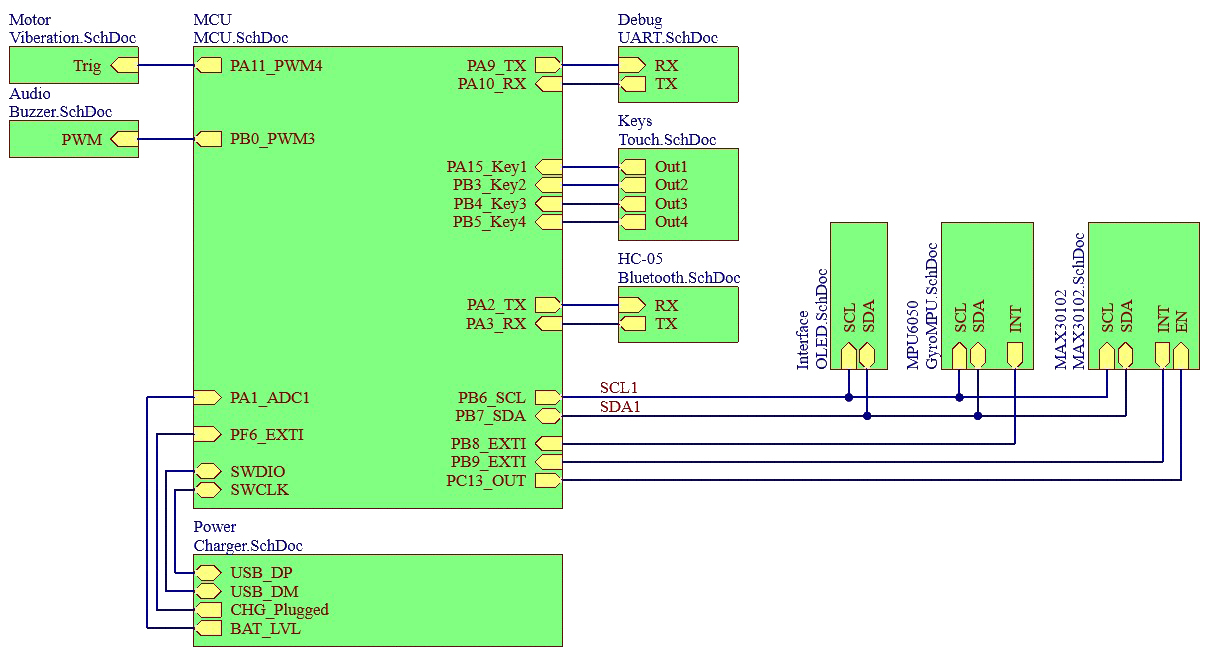
\includegraphics[width=\textwidth]{sch_main}
	\caption{شماتیک کلی ساعت و نحوه‌ی اتصال بخش‌های مختلف به یکدیگر}
	\label{fig:sch-all}
\end{figure}
\section{فیبر مدارچاپی}
	فیبر مدار چاپی یا \pcb\footnote{\lr{Printed Circiut Board}} صفحه‌ای است معمولا از جنس فیبر \lr{FR-4} که با دو لایه‌ی نازک مس (معمولا به ضخامت 35 میکرون) در طرفین پوشیده است. طرحی که طراح به کارخانه‌ی چاپ \pcbf ارسال می‌کند روی این ورقه‌ها پیاده می‌شود. سپس لایه‌ی محافظ معمولا سبز رنگ به نام \lr{Solder mask} روی آن اضافه می‌شود که برای زیبایی بخشی به کار و محافظت از مس در مقابل خوردگی و اکسایش است.
	
	در این پروژه از یک \pcbf چهارلایه استفاده شده است. به دلیل فشردگی بالای طرح و قطعات، همچنین برای بهبود کیفیت سیگنال‌ها و کاهش اثر نویز، دو صفحه‌ی زمین در لایه‌های 2 و 3 تعبیه شده است. این صفحه‌ها با کوتاه کردن مسیر جریان برگشتی باعث بهبود کیفیت سیگنال و کاهش اثر نویز می‌شوند. همچنین تأثیر چشم‌گیری در سهولت مسیرکشی \pcbf دارند.

 \pcbf 
 های این پروژه -به رایگان- توسط شرکت \lr{PCBWay}\cite{PCBWay} چاپ شده است که از بزرگترین و مجهزترین کارخانه‌های چاپ \pcbf در کشور چین است.
 
 شکل \ref{fig:pcb_design}  تصویر \pcbf طراحی شده در نرم‌افزار \lr{Altium Designer} را نشان می‌دهد. تصاویر مربوط به \pcbf در شکل \ref{fig:pcb-images} قابل مشاهده است.
 
 \begin{figure}[h]
 	\centering
 	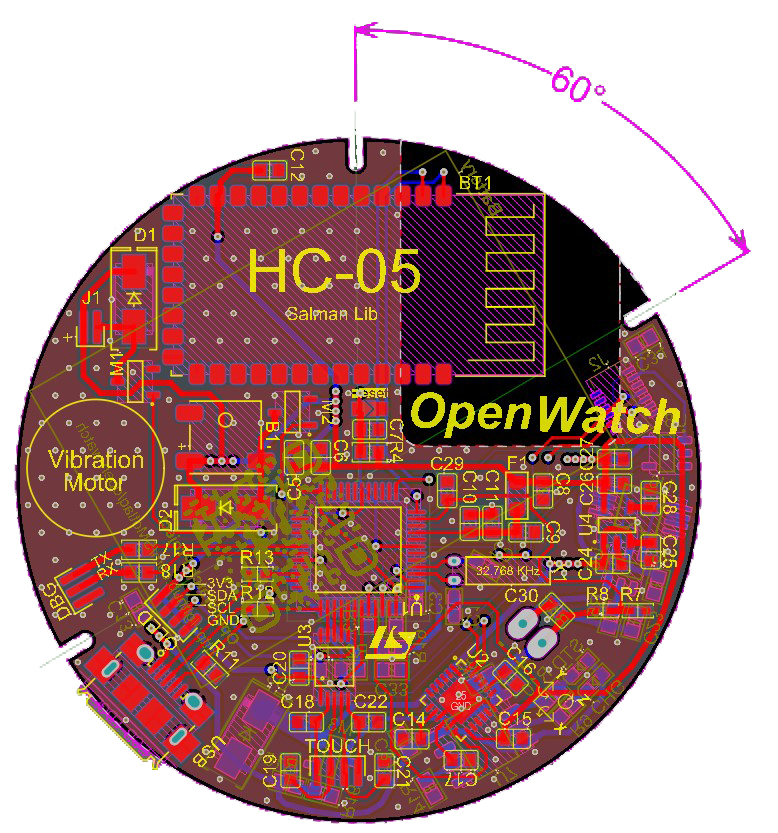
\includegraphics[width=0.6\textwidth]{pcb_main}
 	\caption{\pcbf طراحی شده در نرم‌افزار \lr{Altium Designer}}
 	\label{fig:pcb_design}
 \end{figure}
 
 \begin{figure}[h]
 	\centering
 	\begin{subfigure}{0.45\textwidth}
 		\centering
 		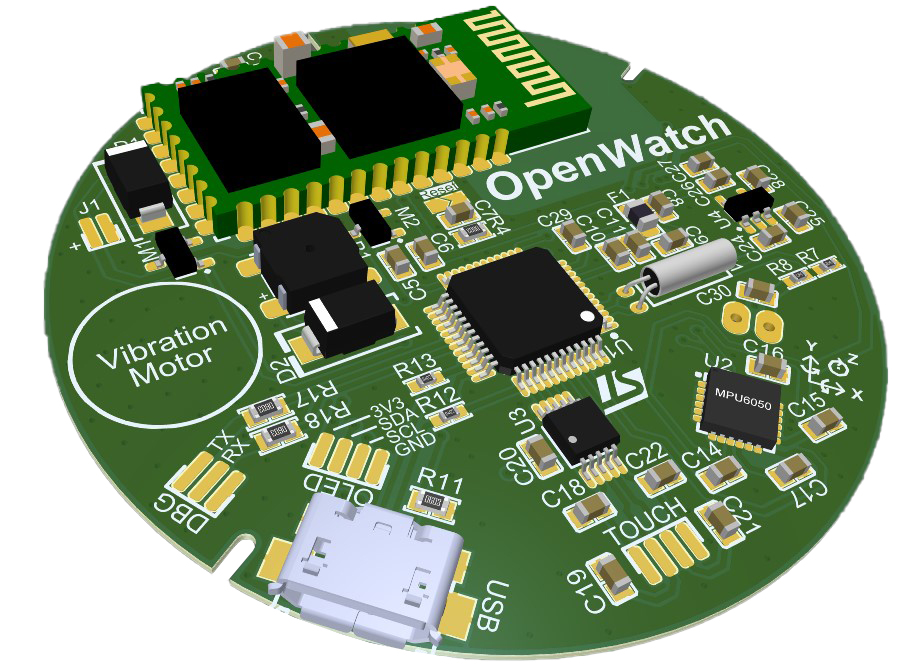
\includegraphics[width=0.9\linewidth]{pcb_main_3d}
 		\caption{نمای سه بعدی طرح - رو}
 		%\label{fig:stm32_image}
 	\end{subfigure}
 	\begin{subfigure}{0.45\textwidth}
 		\centering
 		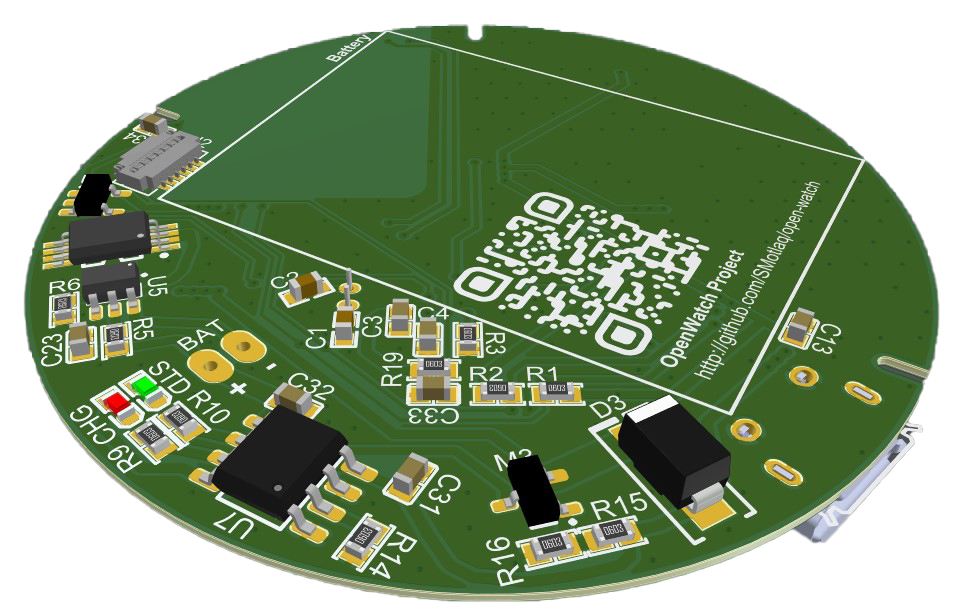
\includegraphics[width=\linewidth]{pcb_main_3d_back}
 		\caption{نمای سه بعدی طرح - پشت}
 		%\label{fig:stm32_real}
 	\end{subfigure}\\
	\begin{subfigure}{0.4\textwidth}
		\centering
		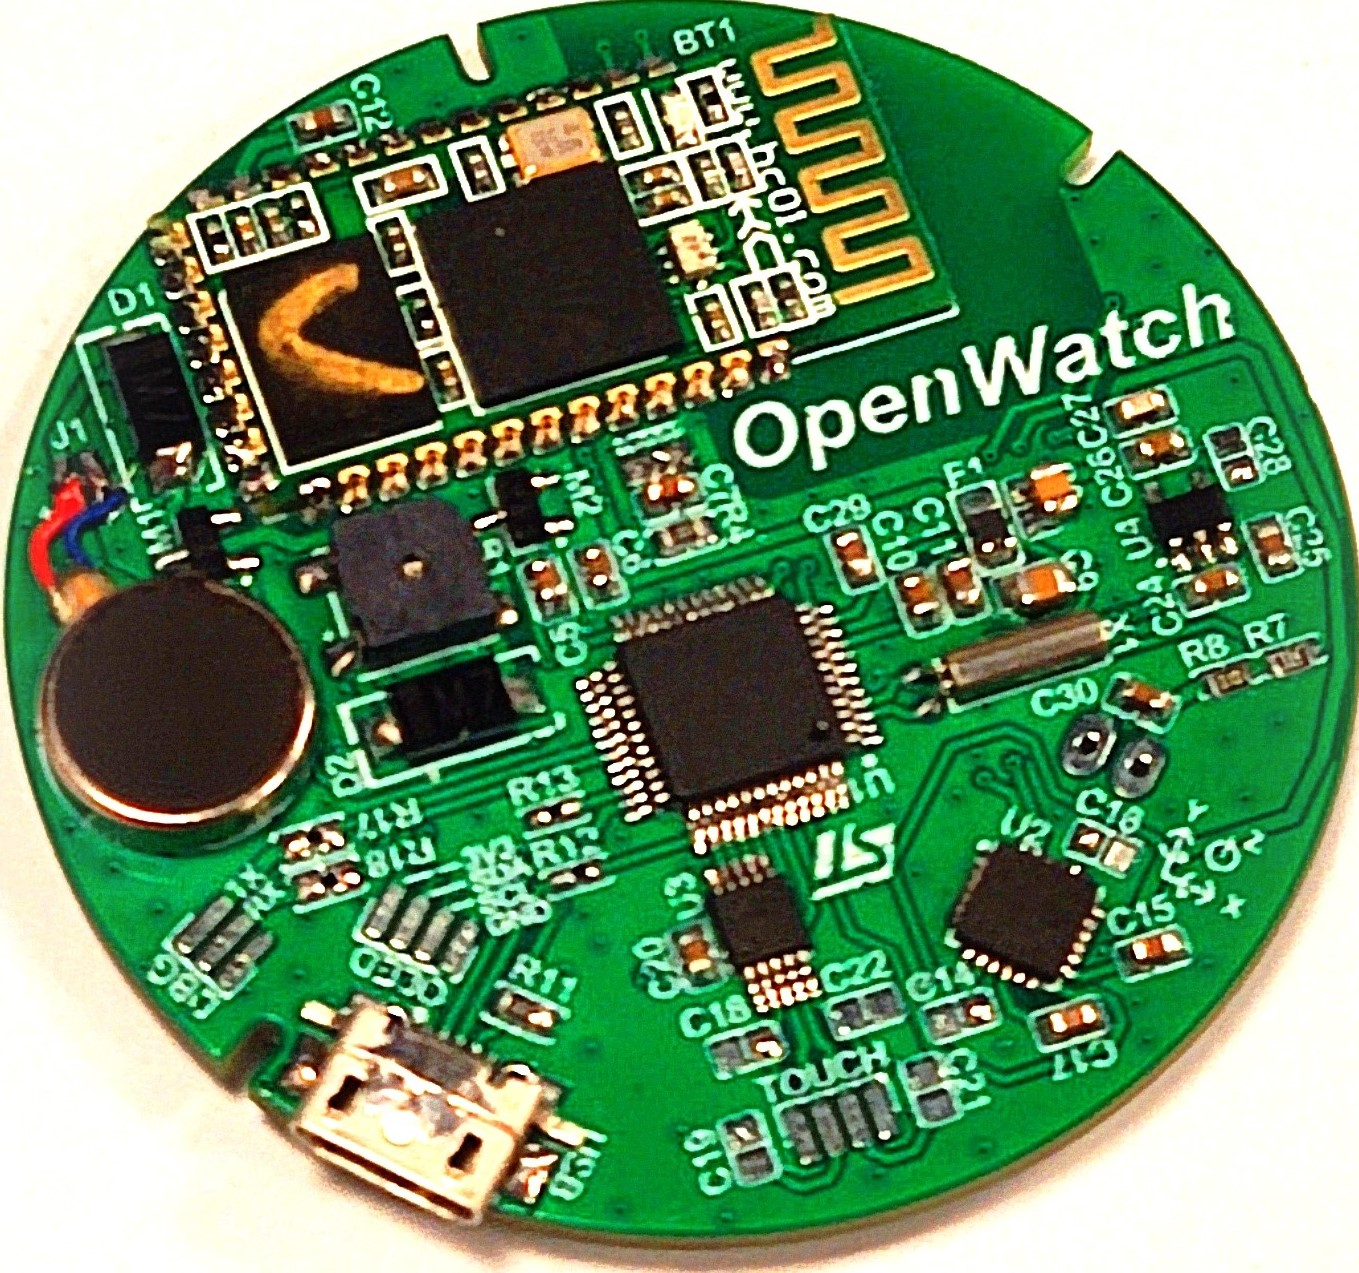
\includegraphics[width=0.9\linewidth]{pcb_real_mounted}
		\caption{\pcbf مونتاژ شده}
		%\label{fig:stm32_image}
	\end{subfigure}
	\begin{subfigure}{0.4\textwidth}
		\centering
		\includegraphics[width=\linewidth]{pcb_real_raw}
		\caption{\pcbf خام}
		%\label{fig:stm32_image}
	\end{subfigure}
 	\caption{تصاویری از \pcbf پروژه}
 	\label{fig:pcb-images}
 \end{figure}
 
\section{هسته‌ی پردازشی} \label{sec:mcu}
برای انتخاب پردازنده‌ی مناسب باید موارد ذیل را مدنظر داشت:
\begin{enumerate}
	\item مقدار حافظه‌ی فلش\footnote{\lr{Flash}}:\\
	برنامه‌ای که برای پردازنده نوشته می‌شود در حافظه‌ی فلش ذخیره می‌شود. پس این حافظه مشخص می‌کند چه حجمی از برنامه در این پردازنده جا می‌شود.
	\item مقدار حافظه‌ی رم\footnote{\lr{RAM}}:\\
	این حافظه، یک حافظه‌ی موقت است که متغیرها، اشاره‌گرها\footnote{\lr{Pointers}}، نقطه‌ی بازگشت توابع و مقادیر ثبات‌ها\footnote{\lr{Registers}} به طور موقت در آن نوشته می‌شود. مقدار رم موردنیاز باید با توجه به حجم متغیرها و پیچیدگی عملیاتی و محاسباتی برنامه تعیین شود.
	\item تعداد پایه‌ها و مدارهای واسط\footnote{\lr{Peripherals}}:\\
	پردازنده‌های مختلف تنوع زیادی در نوع و تعداد مدارهای واسط ارائه می‌دهند. با توجه به تعداد سخت‌افزارهای جانبی، باید تعداد پایه و نوع مدارهای واسط موردنیاز تعیین شود.
	\item پکیج\footnote{\lr{Package}}:\\
	پکیج‌های مختلف نمایانگر شکل ظاهری پردازنده است. برخی پکیج‌ها ابعاد بزرگی دارند و برخی دیگر به قدری کوچک هستند که پایه‌های پردازنده در زیر تراشه تعبیه می‌شوند تا فضای کمتری اشغال کند. در انتخاب پکیج باید محدودیت فضای \pcbf را مدنظر قرار داد.
	\item موجودی بازار:\\
	یکی از مهمترین چالش‌های مهندسان الکترونیک در ایران، موجودی بازار است. خیلی از قطعاتی که طراح به آن‌ها نیاز دارد در بازار ایران پیدا نمی‌شود یا قیمت بالایی دارد. یا باید به وارد کردن قطعه و تاخیر چند ماهه تن داد یا باید طرح را عوض کرد تا با قطعات موجود در بازار قابل پیاده‌سازی باشد.
	\item قیمت:\\
	بدیهی است که یکی از قیود طراحی، قیمت تمام شده است. طراح باید در انتخاب پردازنده طوری عمل کند که با کمترین قیمت، بهترین تطابق را با قیود بالا ایجاد کند.
\end{enumerate}

در نهایت با بررسی موارد فوق، پردازنده‌ی انتخاب شده در این پروژه \lr{STM32F030C8} است. این پردازنده محصول شرکت \lr{ST} که هسته‌ی \lr{ARM Cortex-M0} 32 بیتی دارد. شکل \ref{fig:stm32_image} تصویر واقعی این پردازنده و شکل \ref{fig:stm32_real} تصویر آن را بر روی \pcbf ساعت نشان می‌دهد.

\begin{figure}[h]
	\centering
	\begin{subfigure}{0.35\textwidth}
		\centering
		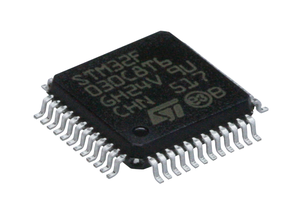
\includegraphics[width=\linewidth]{stm32f030}
		\caption{جداگانه}
		\label{fig:stm32_image}
	\end{subfigure}
	\begin{subfigure}{0.35\textwidth}
		\centering
		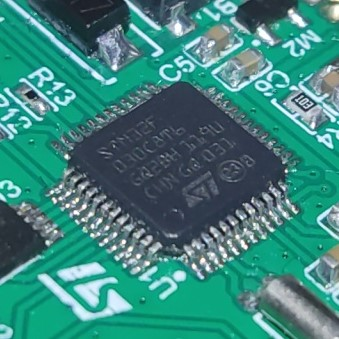
\includegraphics[width=\linewidth]{stm32f030_real}
		\caption{مونتاژ شده روی برد پروژه}
		\label{fig:stm32_real}
	\end{subfigure}
	\caption{تصاویری از پردازنده \lr{STM32F030}}
	\label{fig:stm32}
\end{figure}

شکل \ref{fig:sch-mcu} شماتیک مداری بخش پردازنده را نشان می‌دهد. یک کریستال 32768 هرتزی وظیفه‌ی تنظیم فرکانس بخش
 \lr{RTC}\footnote{\lr{Real Time Clock}}
  را بر عهده دارد. ساعت سیستم توسط این واحد ذخیره و تنظیم می‌شود. تغذیه‌ی بخش 
  \lr{ADC}\footnote{\lr{Analog to Digital Converter}}
  توسط چند خازن و یک فریت‌بید\footnote{\lr{Ferrite Bead}} فیلتر شده است. تغذیه‌ی خود پردازنده نیز توسط 4 خازن (مطابق با دستور کارخانه سازنده) فیلتر شده است.

\begin{figure}
	\centering
	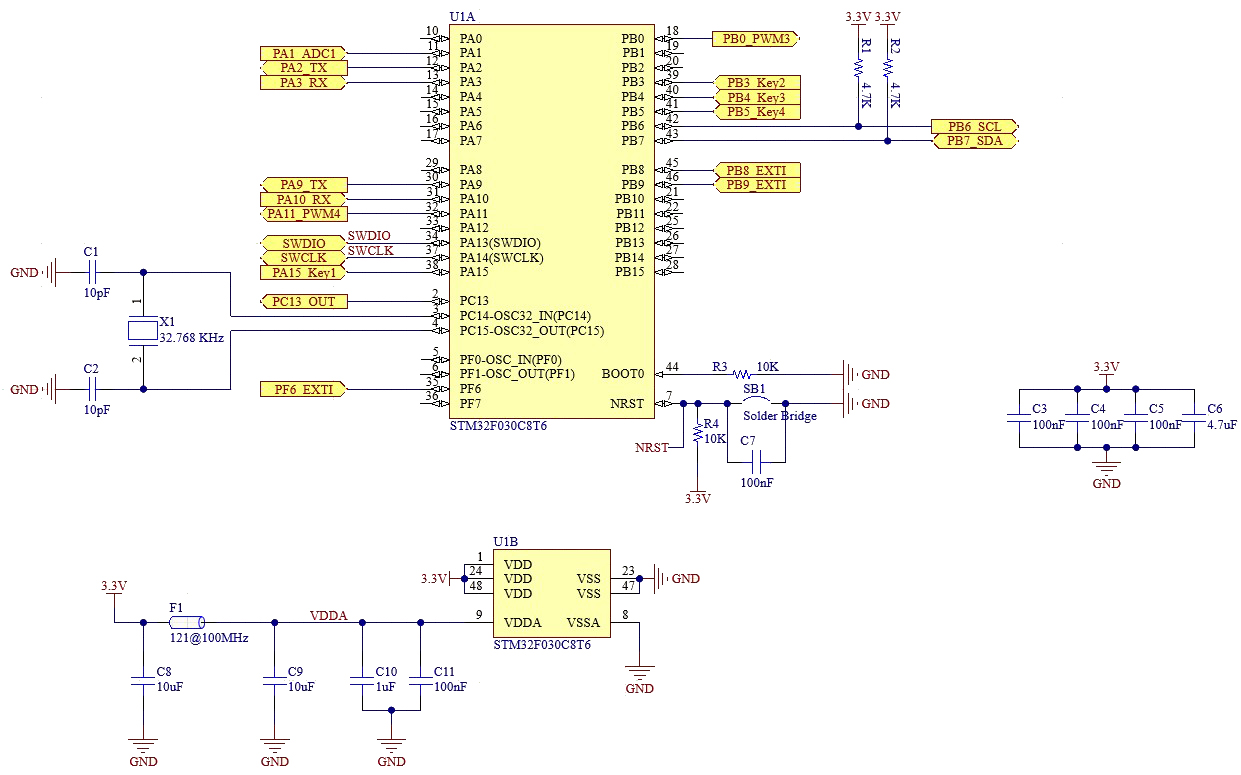
\includegraphics[width=\textwidth]{sch_mcu}
	\caption{شماتیک مربوط به بخش ریزپردازنده}
	\label{fig:sch-mcu}
\end{figure}

\section{درگاه بلوتوث}
ارتباط ساعت با تلفن‌همراه از طریق درگاه بلوتوث\footnote{\lr{Bluetooth}} است. قیود انتخاب بلوتوث هم تا حدی مشابه قیود انتخاب پردازنده (ابتدای بخش \ref{sec:mcu}) است. با در نظر گرفتن شرایط بازار، قیمت و عملکرد ماژول‌های مختلف، نهایتا ماژول \lr{HC-05} برای این پروژه انتخاب شد. شکل \ref{fig:hc05_image} تصویر این ماژول و شکل \ref{fig:hc05_real} تصویر آن را بر روی \pcbf ساعت نشان می‌دهد.

یکی از نکات مهمی که در طراحی \pcbf برای ماژول‌های مخابراتی وجود دارد این است که در نزدیکی آنتن این ماژول‌ها نباید هادی جریان الکتریکی وجود داشته باشد. در غیر این صورت خاصیت خازنی بین آنتن و این هادی باعث تغییر مشخصه‌های آنتن می‌شود و باعث اختلال در عملکرد آنتن می‌گردد. همانطور که در شکل \ref{fig:pcb_design} مشاهده می‌شود، مس‌های اطراف آنتن  حذف شده‌اند تا عملکرد بلوتوث دچار مشکل نشود.

\begin{figure}[h]
	\centering
	\begin{subfigure}{0.4\textwidth}
		\centering
		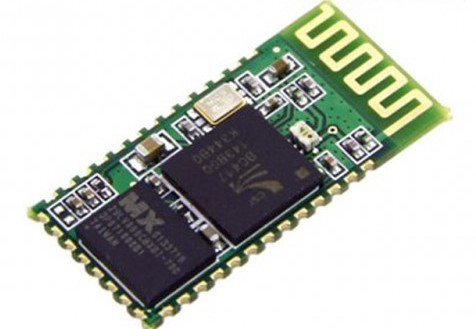
\includegraphics[width=\linewidth]{hc05_real}
		\caption{جداگانه}
		\label{fig:hc05_image}
	\end{subfigure}
	\begin{subfigure}{0.5\textwidth}
		\centering
		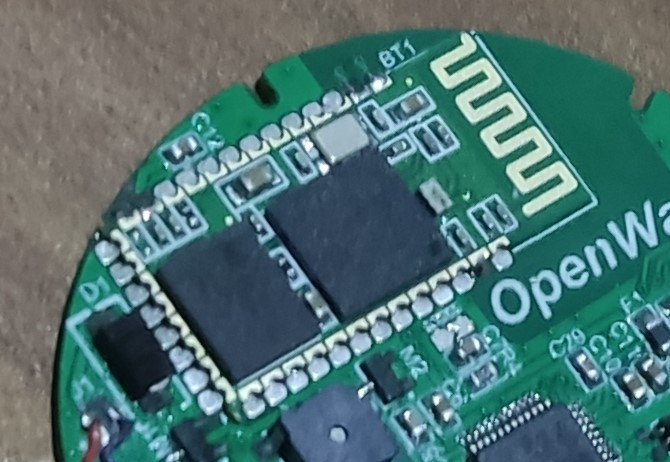
\includegraphics[width=\linewidth]{hc05_mounted}
		\caption{مونتاژ شده روی برد پروژه}
		\label{fig:hc05_real}
	\end{subfigure}
	\caption{تصاویری از ماژول بلوتوث \lr{HC-05}}
	\label{fig:hc05}
\end{figure}

شکل \ref{fig:sch-blue} شماتیک مداری بخش بلوتوث را نشان می‌دهد. پروتکل ارتباطی این ماژول با پردازنده پروتکل
 \lr{UART}\footnote{\lr{Universal Asynchronous Receiver-Transmitter}}
است که با دو پین \lr{RX} و \lr{TX} به پردازنده متصل می‌شود. پریفرال \lr{UART2} در پردازنده به ارتباط با بلوتوث اختصاص دارد. تغذیه‌ی ماژول نیز با یک خازن 100 نانوفارادی فیلتر شده است.

\begin{figure}[h]
	\centering
	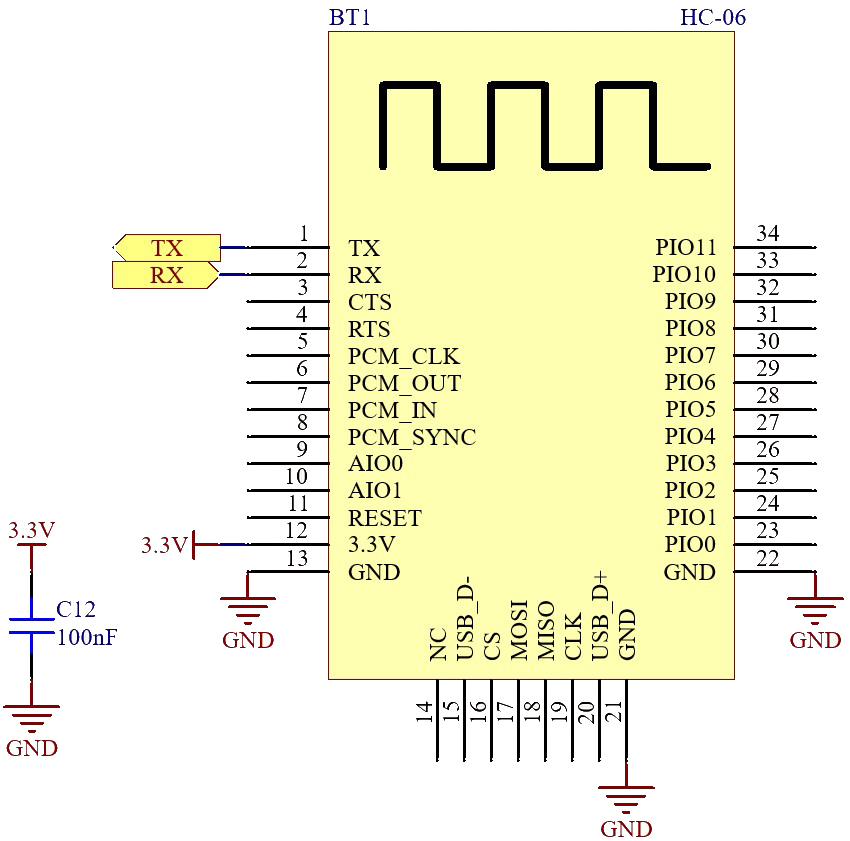
\includegraphics[width=0.6\textwidth]{sch_blue}
	\caption{شماتیک مربوط به بخش بلوتوث}
	\label{fig:sch-blue}
\end{figure}




\section{حسگر شتاب خطی و سرعت زاویه‌ای}
برای اندازه‌گیری مشخصه‌های حرکتی باید سراغ
\lr{IMU}\footnote{\lr{Inertial Measurement Unit}}ها
رفت. \lr{IMU}ها وسیله‌های الکترونیکی هستند که با استفاده‌ی ترکیبی از شتاب‌سنج‌ها، ژیروسکوپ‌ها و گاهی اوقات مغناطیس‌سنج‌ها، مشخصه‌های حرکتی را اندازه‌گیری و گزارش می‌کنند \cite{IMU}. در این پروژه از حسگر \lr{MPU6050} به این منظور استفاده شده است. این حسگر علی‌رغم قیمت نسبتا پایین، دقت و سرعت مناسبی دارد. مشخصات فنی این حسگر در ضمیمه ؟ موجود است. شکل \ref{fig:gyro_image} تصویر این حسگر و شکل \ref{fig:gyro_real} تصویر آن را بر روی \pcbf ساعت نشان می‌دهد.

\begin{figure}[h]
	\centering
	\begin{subfigure}{0.5\textwidth}
		\centering
		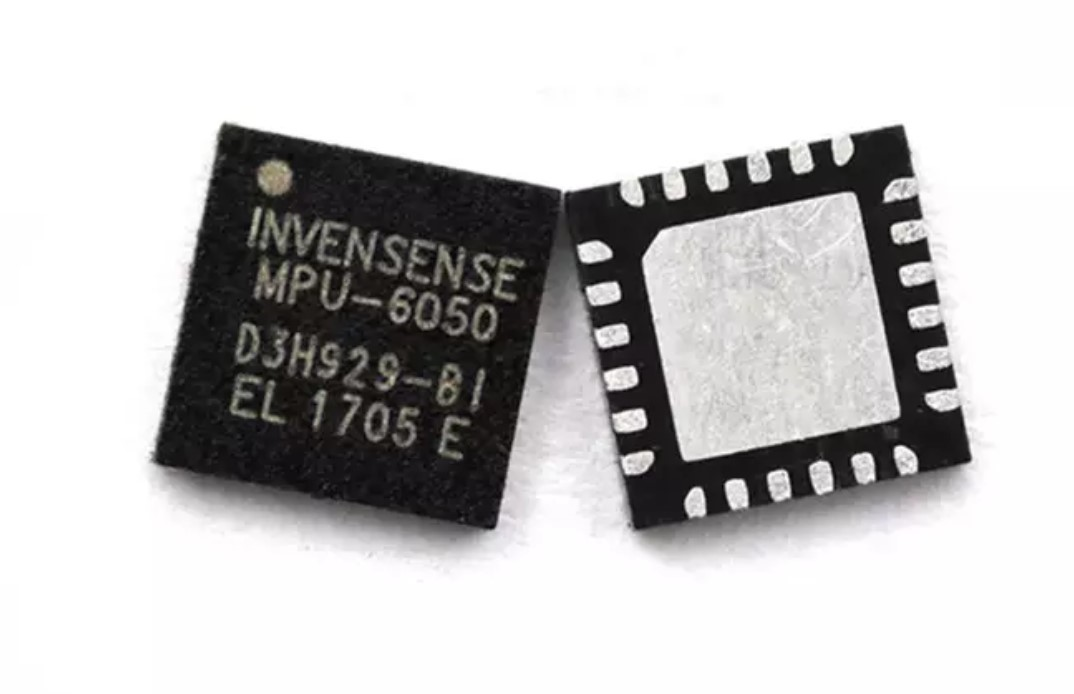
\includegraphics[width=\linewidth]{gyro_image}
		\caption{جداگانه}
		\label{fig:gyro_image}
	\end{subfigure}
	\begin{subfigure}{0.44\textwidth}
		\centering
		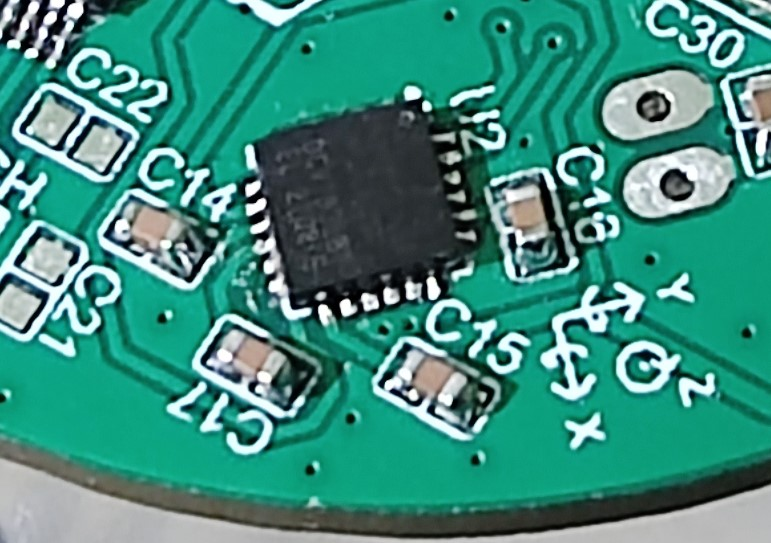
\includegraphics[width=\linewidth]{gyro_real}
		\caption{مونتاژ شده روی برد پروژه}
		\label{fig:gyro_real}
	\end{subfigure}
	\caption{تصاویر حسگر حرکتی}
	%	\label{fig:hc05}
\end{figure}

شکل \ref{fig:sch-gyro} شماتیک مداری حسگر \lr{MPU6050} را نشان می‌دهد. خازن‌ها طبق دستور کارخانه به حسگر متصل شده‌اند. درگاه ارتباطی این حسگر، باس \lr{I2C} است. به همین دلیل \lr{I2C1} پردازنده به این حسگر متصل است.

\begin{figure}[h]
	\centering
	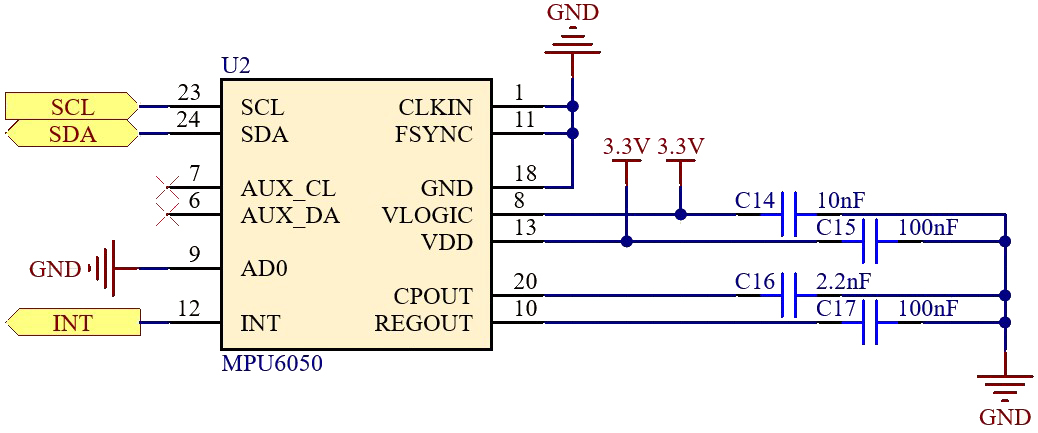
\includegraphics[width=0.95\textwidth]{sch_gyro}
	\caption{شماتیک مربوط به بخش حسگر حرکتی}
	\label{fig:sch-gyro}
\end{figure}

\section{حسگر \lr{PPG}}
در ابتدا ساختار کلی حسگرهای
\lr{PPG}\footnote{\lr{Photoplethysmogram} یا تغییرحجم‌سنجی نوری}
را بررسی می‌کنیم. این حسگرها شامل یک یا چند دیود نشردهنده‌ی نور\footnote{\lr{Light-emitting diode (LED)}} هستند که به همراه گیرنده‌ی نوری در یک بسته قرار دارند. وظیفه‌ی این حسگرها این است که نوری را به داخل بافت بدن بفرستند و بازتاب آن را دریافت کنند. با پردازش سیگنال دریافتی می‌توان به اطلاعاتی مانند ضربان قلب و سطح اکسیژن خون دست یافت.

بسته به کاربرد موردنظر، نورهای مختلفی در این سنسورها استقاده می‌شود. حسگر استفاده شده در این پروژه \lr{MAX30102} نام دارد. این حسگر دارای دو نور قرمز و مادون قرمز است. ساختار منعطف این حسگر کمک می‌کند تا بتوان به سادگی آن را در بدنه نصب کرد. متاسفانه این حسگر در بازار ایران موجود نبود و مجبور به وارد کردن آن از چین شدم. تصویر این حسگر در شکل \ref{fig:ppg_image} و محل اتصال آن روی \pcbf در شکل \ref{fig:ppg_real} قابل مشاهده است.

\begin{figure}[h]
	\centering
	\begin{subfigure}{0.45\textwidth}
		\centering
		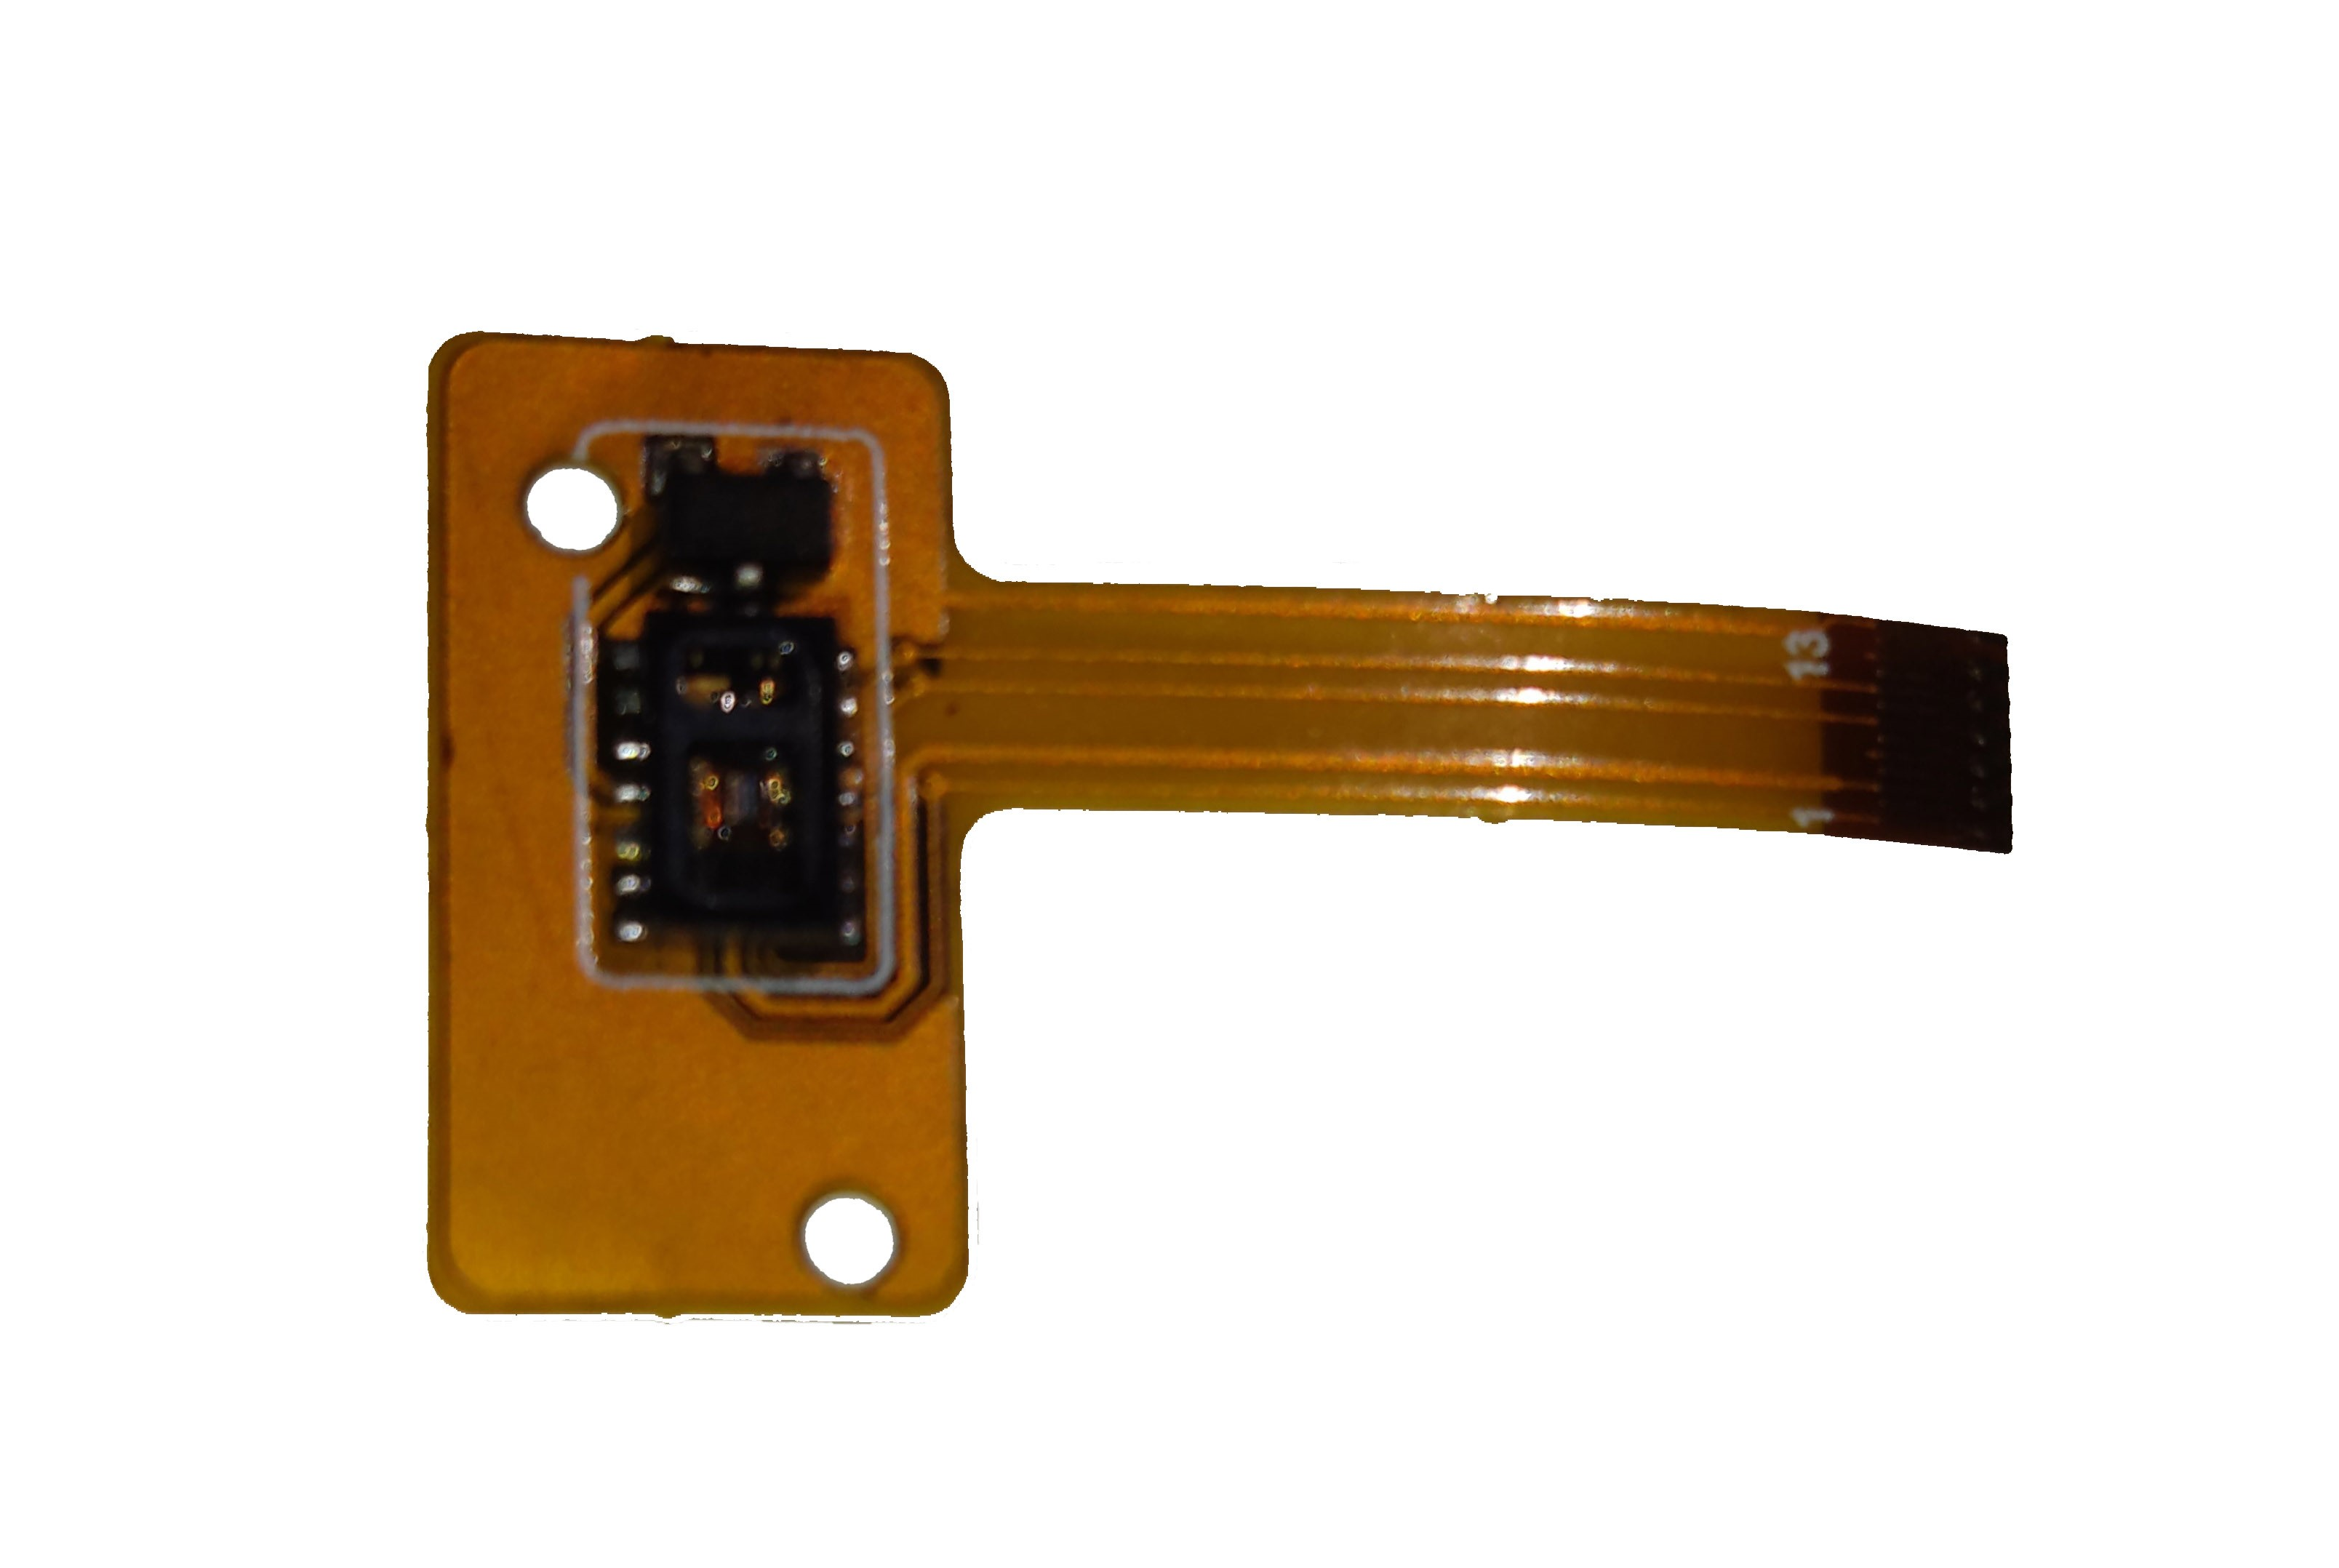
\includegraphics[width=\linewidth]{ppg_image}
		\caption{جداگانه}
		\label{fig:ppg_image}
	\end{subfigure}
	\begin{subfigure}{0.35\textwidth}
		\centering
		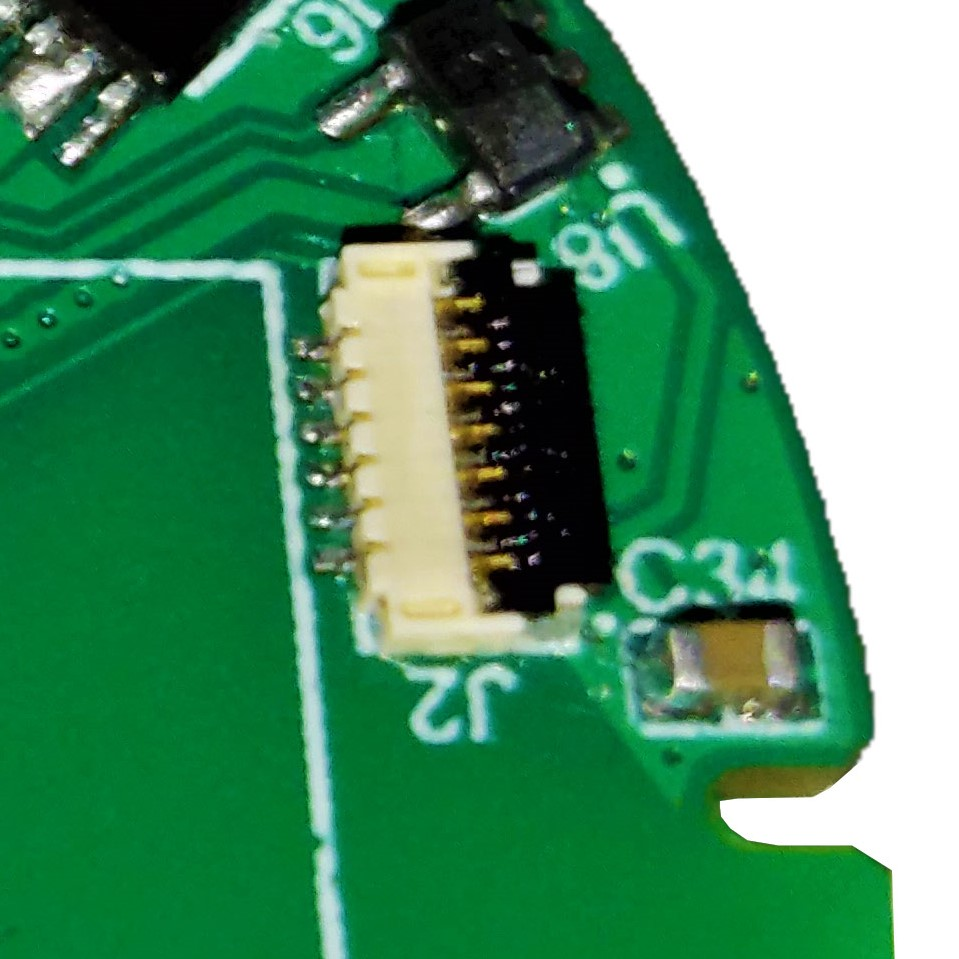
\includegraphics[width=0.9\linewidth]{ppg_real}
		\caption{محل اتصال حسگر روی برد پروژه}
		\label{fig:ppg_real}
	\end{subfigure}
	\caption{تصاویر حسگر \lr{PPG}}
	%	\label{fig:hc05}
\end{figure}

شکل \ref{fig:sch-ppg} شماتیک مداری حسگر \lr{MAX30102} را نشان می‌دهد. همانطور که دیده می‌شود یک آیسی \lr{RT9742GGJ5} بر سر راه تغذیه‌ی سنسور قرار دارد. این آیسی یک سوییچ ماسفت\footnote{\lr{Metal–Oxide–Semiconductor Field-Effect Transistor}} است که علاوه بر قطع و وصل تغذیه، مصرف کننده را در مقابل مواردی چون کمبود ولتاژ، اضافه جریان و افزایش دما محافظت می‌کند. از آنجا که نیازی نیست این حسگر دائما روشن باشد و نمونه برداری کند، این سوییچ کمک می‌کند تا بتوان حسگر را روشن یا خاموش کرد.

کانکتوری که برای حسگر استفاده شده یک کانکتور \lr{FPC} 13 پین است که متاسفانه آن هم در بازار ایران موجود نبود و وارد شد.
درگاه ارتباطی این حسگر، باس\footnote{\lr{Bus}}
\lr{I2C}\footnote{\lr{Inter-Integrated Circiut}}
است. به همین دلیل \lr{I2C1} پردازنده به این حسگر متصل است.

\begin{figure}[h]
	\centering
	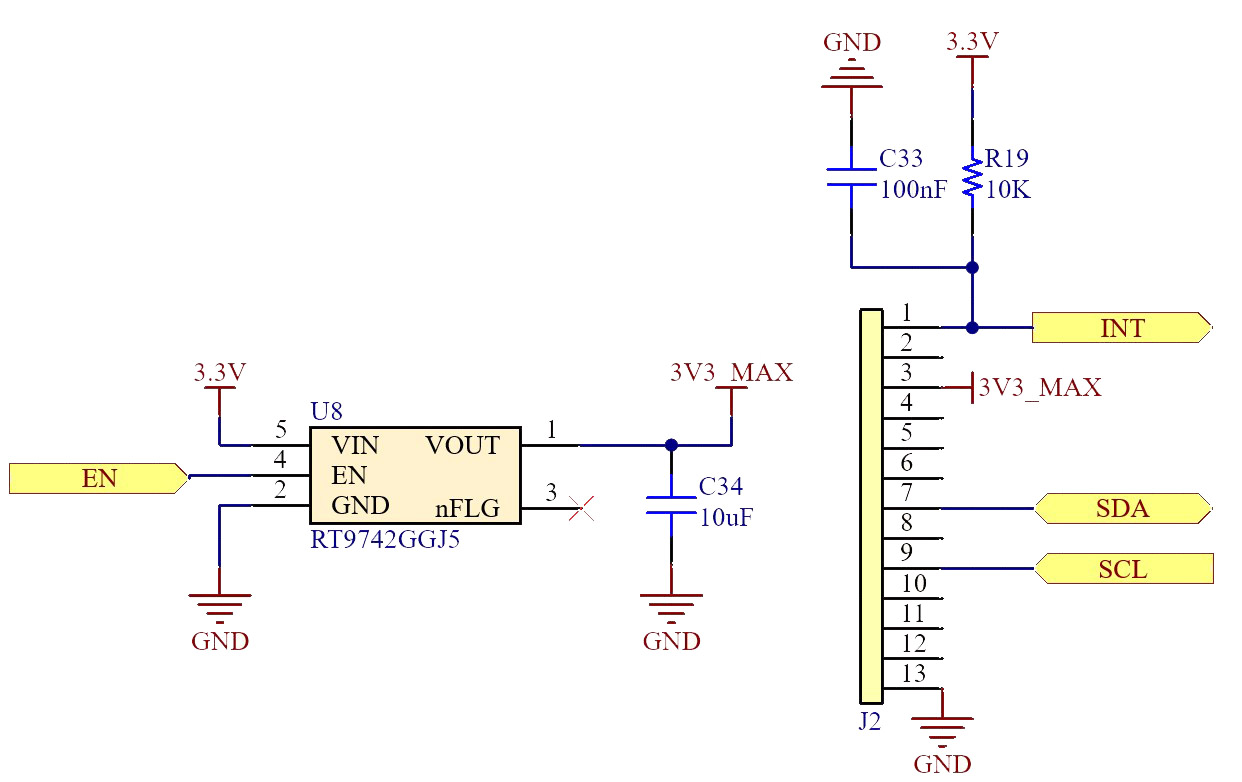
\includegraphics[width=0.7\textwidth]{sch_ppg}
	\caption{شماتیک مربوط به بخش حسگر \lr{PPG}}
	\label{fig:sch-ppg}
\end{figure}


\section{صفحه نمایش}
صفحه‌ی نمایش از اصلی‌ترین قسمت‌های یک ساعت هوشمند است. صفحه‌ی نمایش باید مصرف کمی داشته باشد، راه‌اندازی آن دشوار نباشد و تعداد پایه‌ی زیادی هم نیاز نداشته باشد تا بتوان آن را در ساعت استفاده کرد. از این رو یک صفحه‌ی نمایش\lr{OLED}\footnote{صفحه‌ی نمایش‌های \lr{OLED} اینگونه هستند که فقط پیکسل‌های موردنیاز روشن می‌شوند و دیگر نیازی نیست که نور پشتی به تمام پیکسل‌ها بتابد تا دیده شوند. این نوع نمایشگرها مصرف کمتر و زیبایی بیشتری دارند.} 3.1 اینچی با ابعاد 64 در 128 پیکسل انتخاب شد که به کمک درایور \lr{SSD1306} راه‌اندازی می‌شود. شکل \ref{fig:oled_image} تصویر این نمایشگر و شکل \ref{fig:oled_real} تصویر محل اتصال سیم‌های آن را بر روی \pcbf ساعت نشان می‌دهد.

\begin{figure}[h]
	\centering
	\begin{subfigure}{0.44\textwidth}
		\centering
		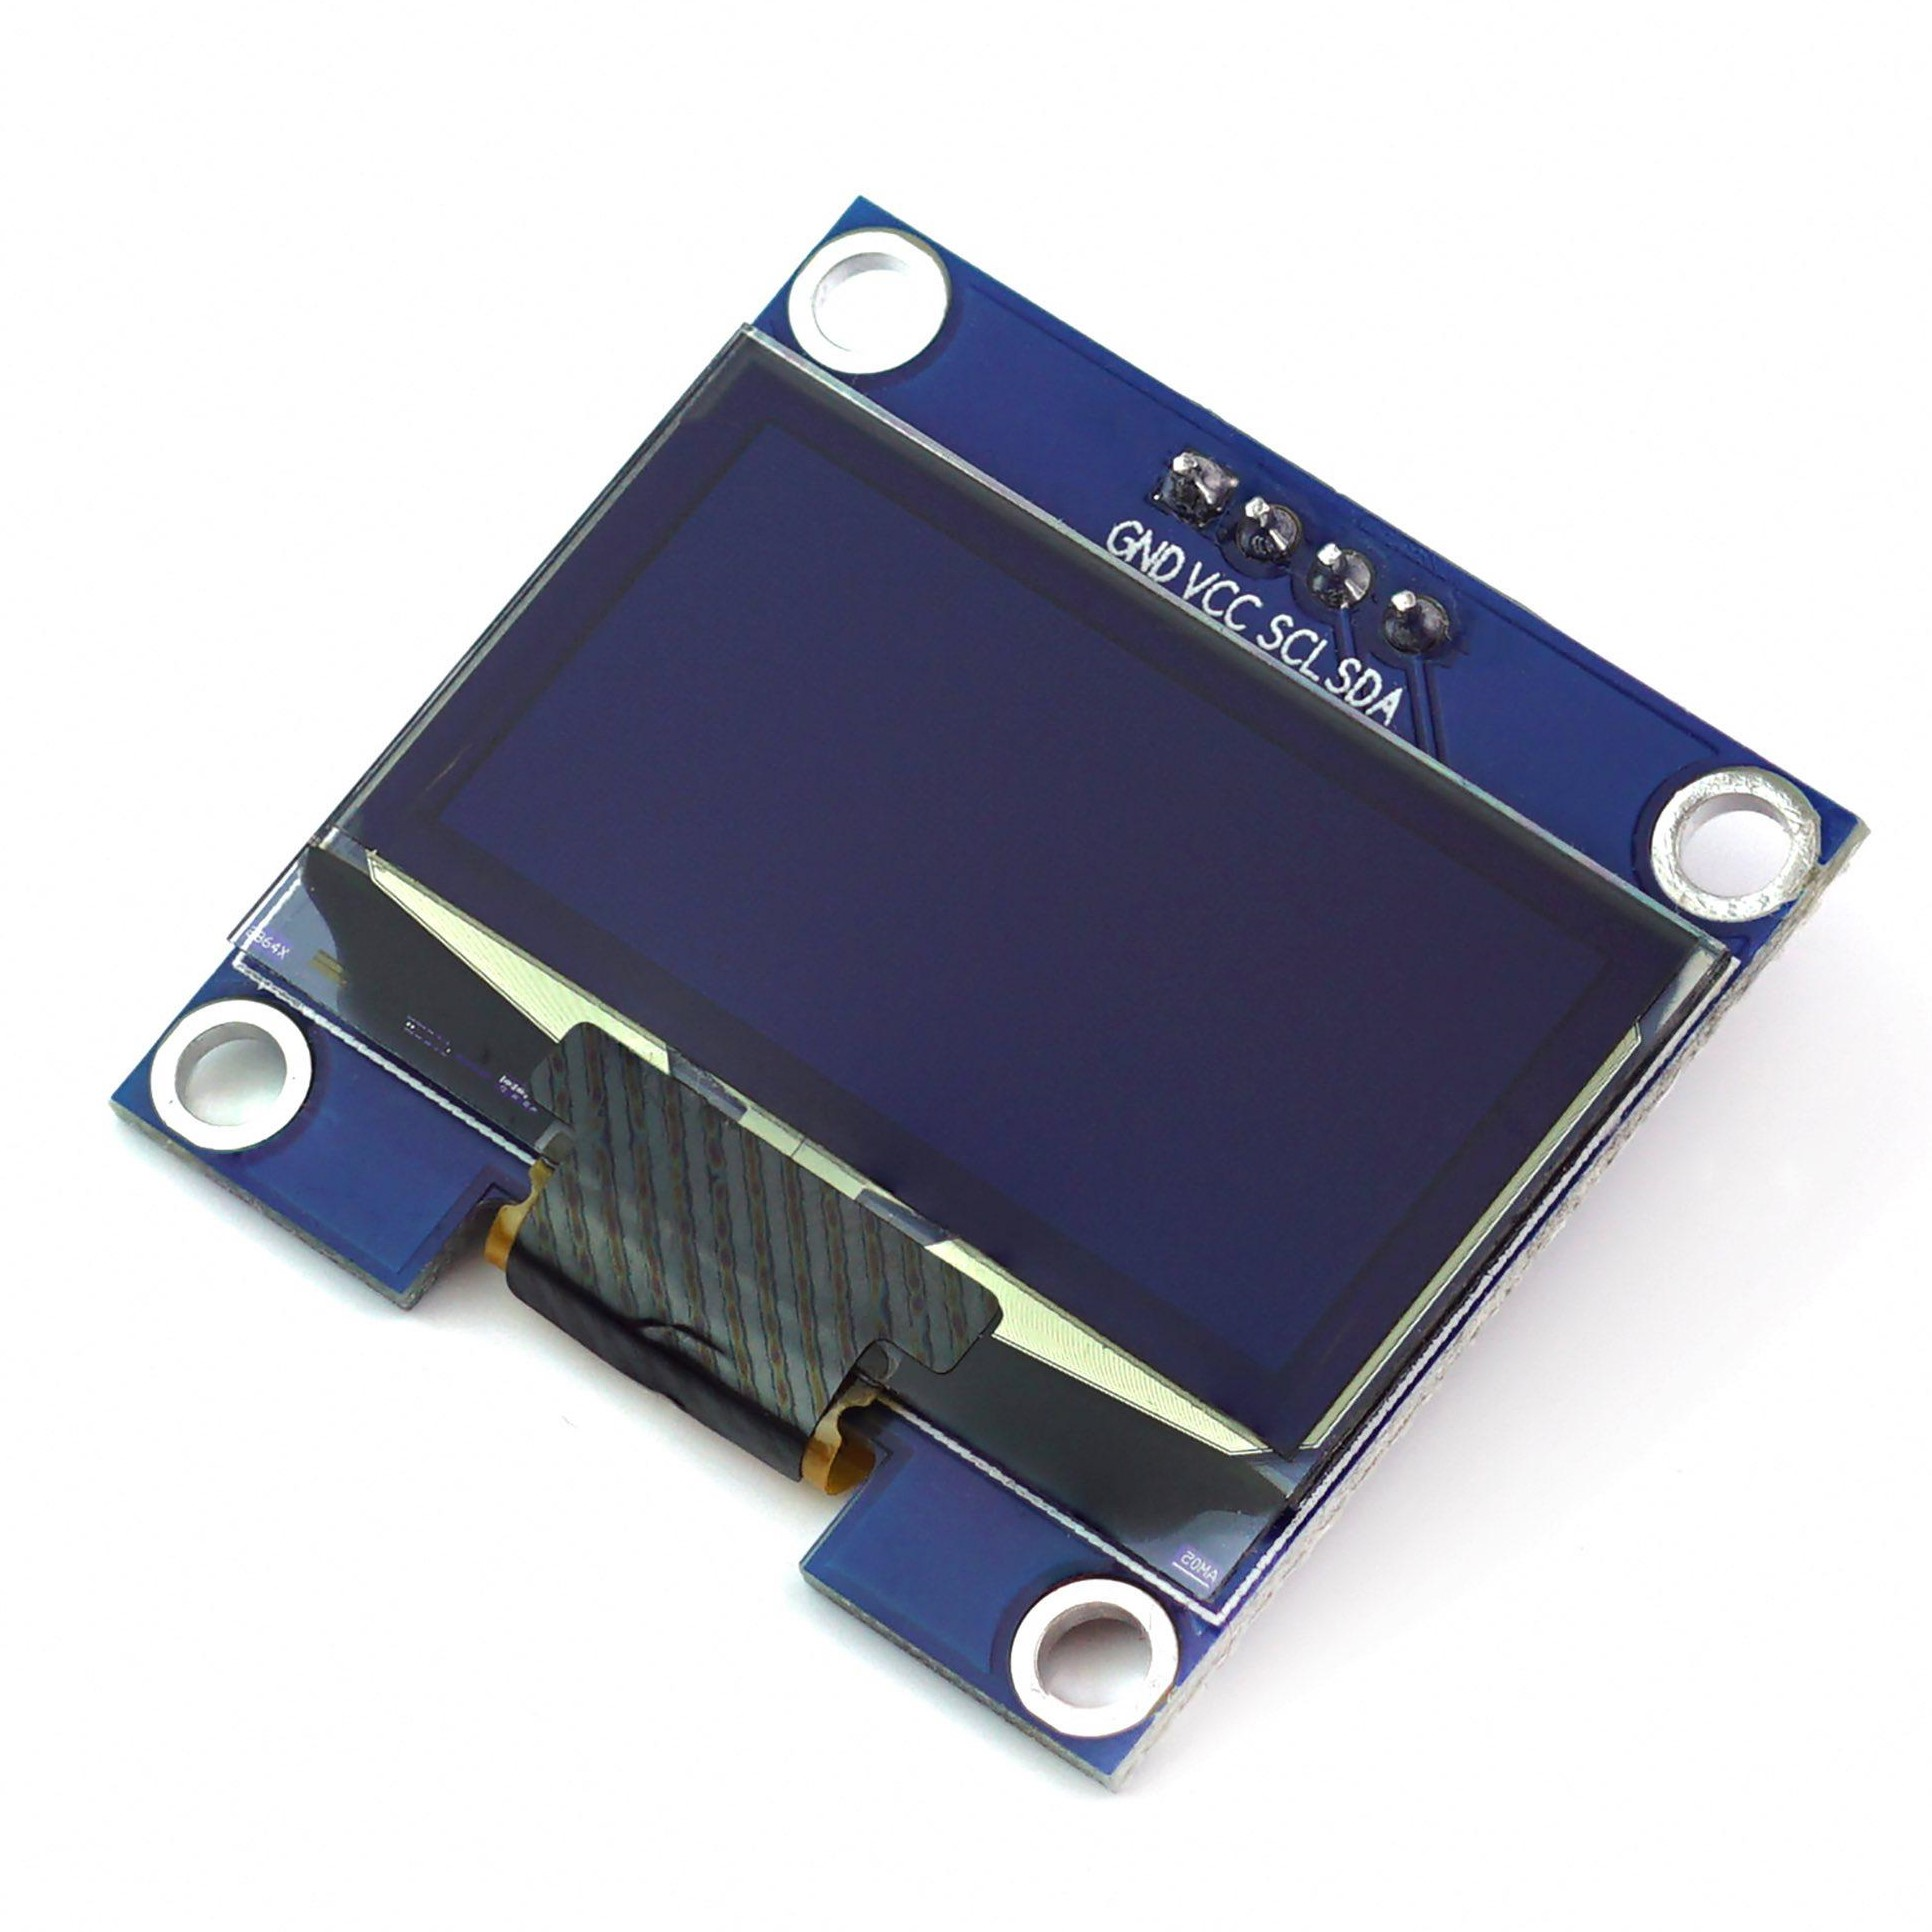
\includegraphics[width=\linewidth]{oled_image}
		\caption{جداگانه}
		\label{fig:oled_image}
	\end{subfigure}
	\begin{subfigure}{0.44\textwidth}
		\centering
		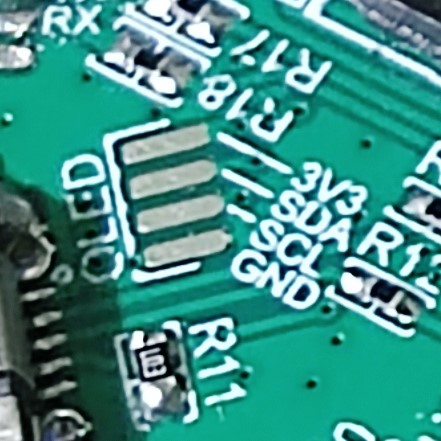
\includegraphics[width=\linewidth]{oled_real}
		\caption{محل اتصال نمایشگر روی برد پروژه}
		\label{fig:oled_real}
	\end{subfigure}
	\caption{تصاویر صفحه‌ی نمایش}
	%	\label{fig:hc05}
\end{figure}

شکل \ref{fig:sch-oled} شماتیک مداری بخش نمایشگر را نشان می‌دهد. درگاه ارتباطی این نمایشگر، باس \lr{I2C} است. به همین دلیل \lr{I2C1} پردازنده به این نمایشگر متصل است.

\begin{figure}[h]
	\centering
	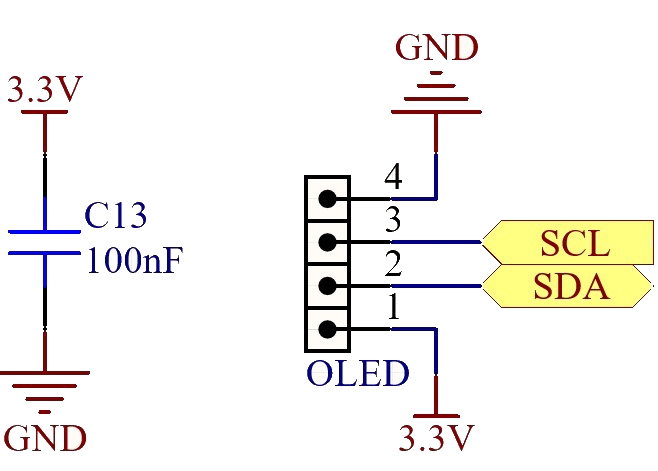
\includegraphics[width=0.6\textwidth]{sch_oled}
	\caption{شماتیک مربوط به بخش نمایشگر}
	\label{fig:sch-oled}
\end{figure}

\section{درگاه ارتباط سریال}

پریفرال \lr{UART1} در پردازنده با دو پین \lr{RX} و \lr{TX} از روی \pcbf خارج شده‌اند. کاربرد این دو پین اشکال‌یابی\footnote{\lr{Debug}} و ارتباط سرعت بالا بین ساعت و رایانه است. این بخش کاربردی در عملکرد کلی ساعت ندارد و صرفا روند توسعه را تسریع می‌کند. شکل \ref{fig:sch_debug} شماتیک مداری و شکل \ref{fig:debug_real} تصویر واقعی این دو پین را نشان می‌دهد.

\begin{figure}[h]
	\centering
	\begin{subfigure}{0.59\textwidth}
		\centering
		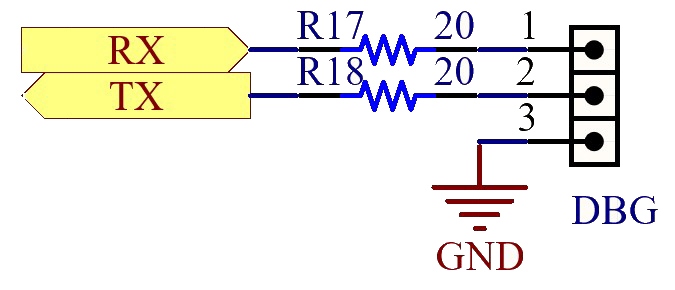
\includegraphics[width=\linewidth]{sch_debug}
		\caption{شماتیک}
		\label{fig:sch_debug}
	\end{subfigure}
	\begin{subfigure}{0.4\textwidth}
		\centering
		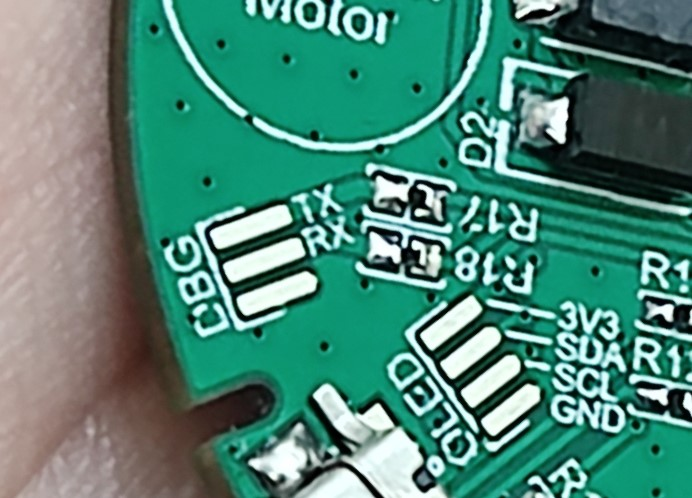
\includegraphics[width=\linewidth]{debug_real}
		\caption{پین‌های مربوطه}
		\label{fig:debug_real}
	\end{subfigure}
	\caption{تصاویر مربوط به درگاه ارتباط سریال}
\end{figure}

\section{تغذیه و مدیریت توان}
بخش تغذیه و مدیریت توان این ساعت هوشمند از دو قسمت تشکیل شده است. بخش تغذیه که شامل باتری است و بخش شارژ که وظیفه‌ی شارژ باتری و تغذیه‌ی مدار را در صورت اتصال شارژر بر عهده دارد.

\subsection{باتری}
برای انتخاب باتری قیودی چون ظرفیت، ولتاژ، ابعاد و قیمت مطرح است. باتری‌ای برای این پروژه مناسب است که در حداقل ابعاد، حداکثر ظرفیت را داشته باشد، در بازار موجود باشد، قیمت مناسبی داشته باشد و یک سلول باشد (ولتاژ 7.3 ولت). با این تفاسیر باتری‌ای که در شکل \ref{fig:battery} مشاهده می‌شود برای این پروژه انتخاب شد. یک باتری لیتیوم-یون یک سلولی که ولتاژ نامی آن 7.3 ولت است با ظرفیت 400 میلی‌آمپرساعت.

\begin{figure}[h]
	\centering
	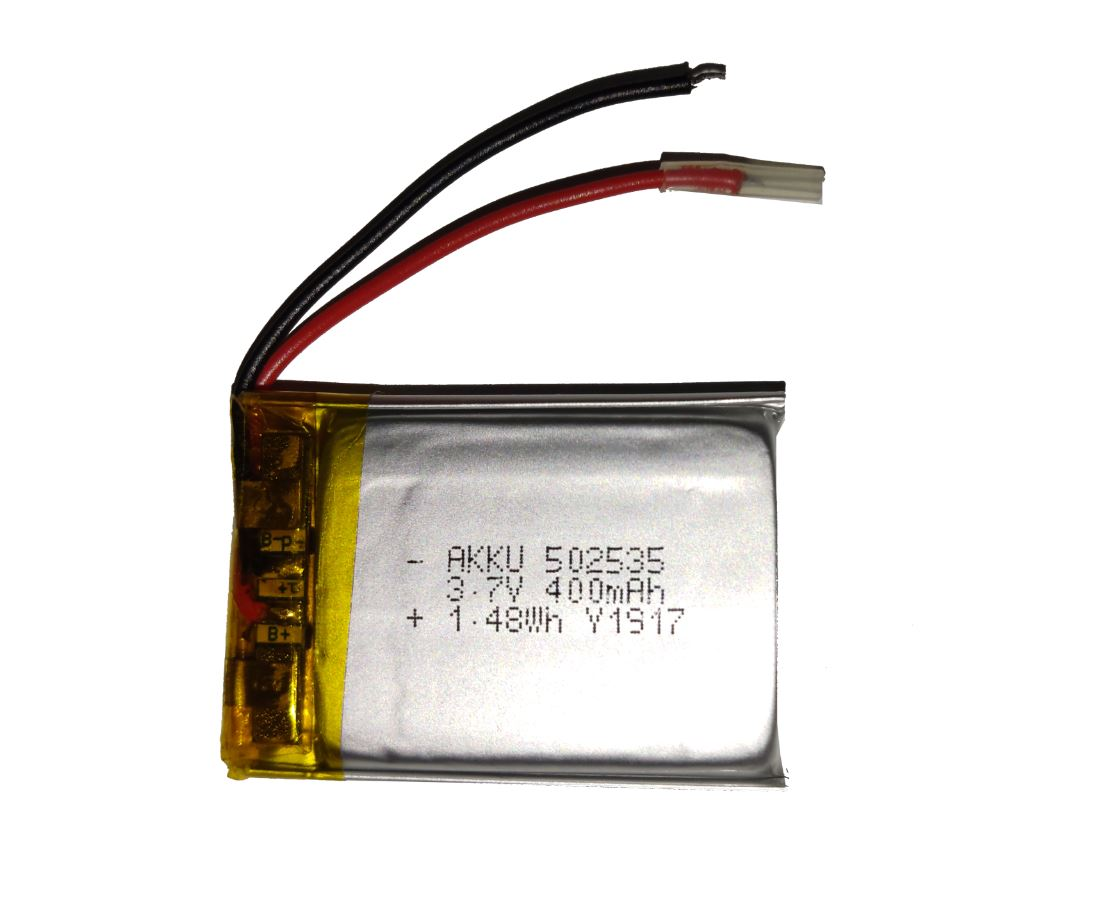
\includegraphics[width=0.7\textwidth]{battery}
	\caption{باتری انتخاب شده برای پروژه}
	\label{fig:battery}
\end{figure}

\subsection{شارژ و مدیریت توان}
برای شارژ باتری از یک آیسی شارژ به نام \lr{TP4056} استفاده شده است که می‌تواند باتری‌های لیتیومی را شارژ کند. در کنار آن یک آیسی کنترلر به نام \lr{DW01} قرار دارد که ولتاژ باتری را پایش می‌کند. باتری های یک سلولی ولتاژ نامی 7.3 ولت دارند. اما در حالت شارژ کامل حدود 2.4 و در حالت خالی حدود 3 ولت هستند. این کنترلر وظیفه دارد در صورت تجاوز ولتاژ باتری از این محدوده، آن را به کمک دو ماسفت از مدار خارج کند. اینگونه باتری هیچگاه دچار اضافه ولتاژ\footnote{\lr{Over voltage}} یا کمبود ولتاژ\footnote{\lr{Under voltage}} نمی‌شود و آسیبی نمی‌بیند. این مدارات در شکل \ref{fig:charge} قابل مشاهده‌اند.

تغذیه‌ی مدارهای ساعت از یک رگولاتور 3.3 ولت تأمین می‌شود. بحث مدیریت توان به این مسئله می‌پردازد که ورودی این رگولاتور از کدام مسیر تغذیه شود. هنگامی که باتری شارژ دارد و شارژر متصل نیست، باید ورودی باتری مستقیما به رگولاتور وارد شود. هنگامی که شارژر متصل می‌شود، باید ورودی برق شارژر مستقیما به رگولاتور برود و باتری از مدار خارج شود که از طریق برق ورودی شارژ شود. این تغییر مسیر و جابجایی توسط یک ماسفت \lr{AO3401} صورت می‌گیرد.

این ماسفت یک ماسفت \lr{P-Channel} است. در صورتی هدایت می‌کند که شرط 9.0-
\lr{$V_{GS}<V_{th}=$}
برقرار باشد. حال به شکل \ref{fig:sup-switch} توجه کنید. در صورتی که برق ورودی (5 ولت) متصل باشد، ولتاژ گیت 5 ولت می‌شود. از طرفی ورودی رگولاتور از طریق دیود \lr{D2} که شاتکی است و 2.0 ولت افت دارد، متصل شده است. در این صورت
\lr{$V_{GS}$}
2.0 ولت است و باعث می‌شود که ماسفت قطع شود. در این حالت ولتاژ سورس حدود 8.4 است. از آنجا که ولتاژ باتری نهایتا 3.4 ولت است لذا دیود داخلی ماسفت نیز هدایت نمی‌کند و همه چیز درست است. حال اگر تغذیه‌ی خارجی قطع شود؛ گیت ماسفت به دلیل وجود مقاومتِ \lr{Pull-Down} صفر می‌شود. اکنون کافی است تا ولتاژ سورس اندکی مثبت شود (حدود 9.0 ولت) تا ماسفت هدایت کند. این ولتاژ از طریق دیود داخلی ماسفت از سمت باتری ایجاد می‌شود. حالا ماسفت روشن است و ورودی رگولاتور از طریق باتری تغذیه می‌شود. 

\begin{figure}[h]
	\centering
	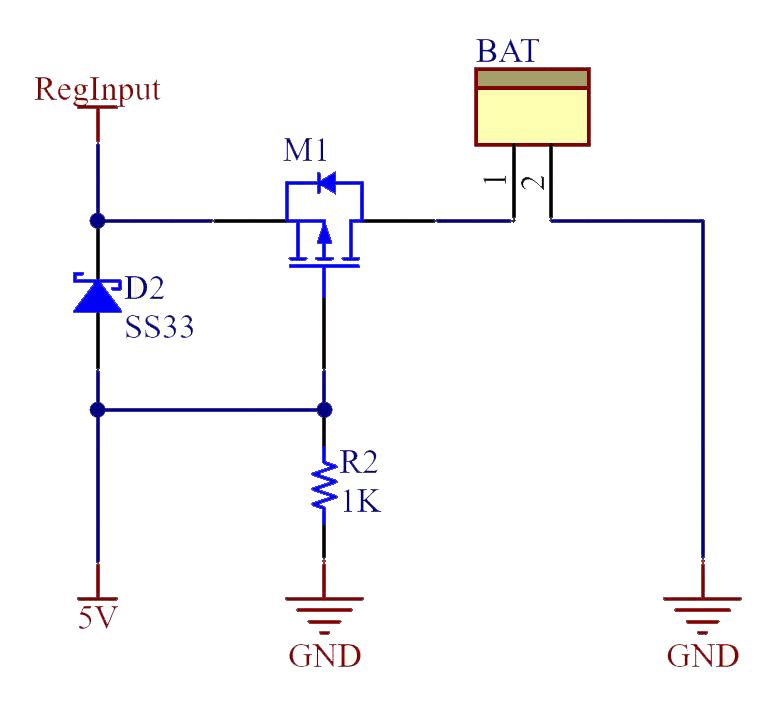
\includegraphics[width=0.45\textwidth]{sup_switch}
	\caption{شماتیکی ساده برای توضیح بخش مدیریت توان}
	\label{fig:sup-switch}
\end{figure}

به طور خلاصه می‌توان حالات کاری مدار را اینگونه توضیح داد:
\begin{enumerate}
	\item شارژر متصل است: ماسفت خاموش است، باتری از مدار خارج شده و به شارژر متصل است
	\item 	شارژر متصل نیست: ماسفت روشن است، باتری در مدار است و به شارژر متصل نیست 
\end{enumerate}

\begin{figure}[h!]
	\centering
	\begin{subfigure}{\textwidth}
		\centering
		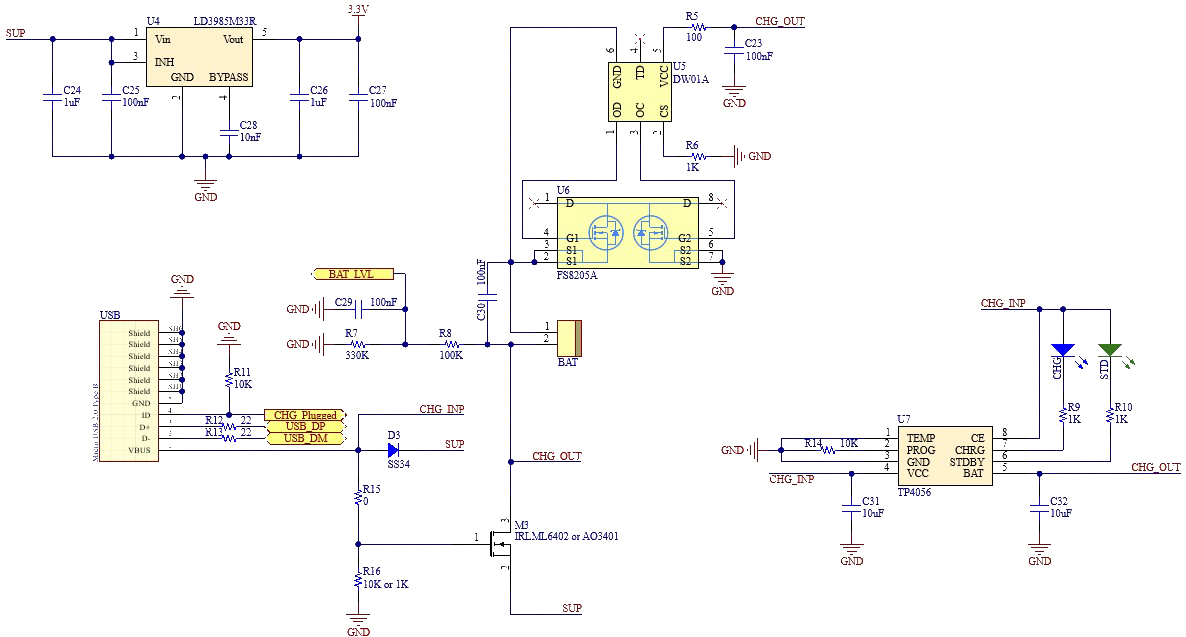
\includegraphics[width=\linewidth]{sch_charg}
		\caption{شماتیک مدار شارژ و مدیریت توان}
		%\label{fig:vib_image}
	\end{subfigure}\\
	\begin{subfigure}{\textwidth}
		\centering
		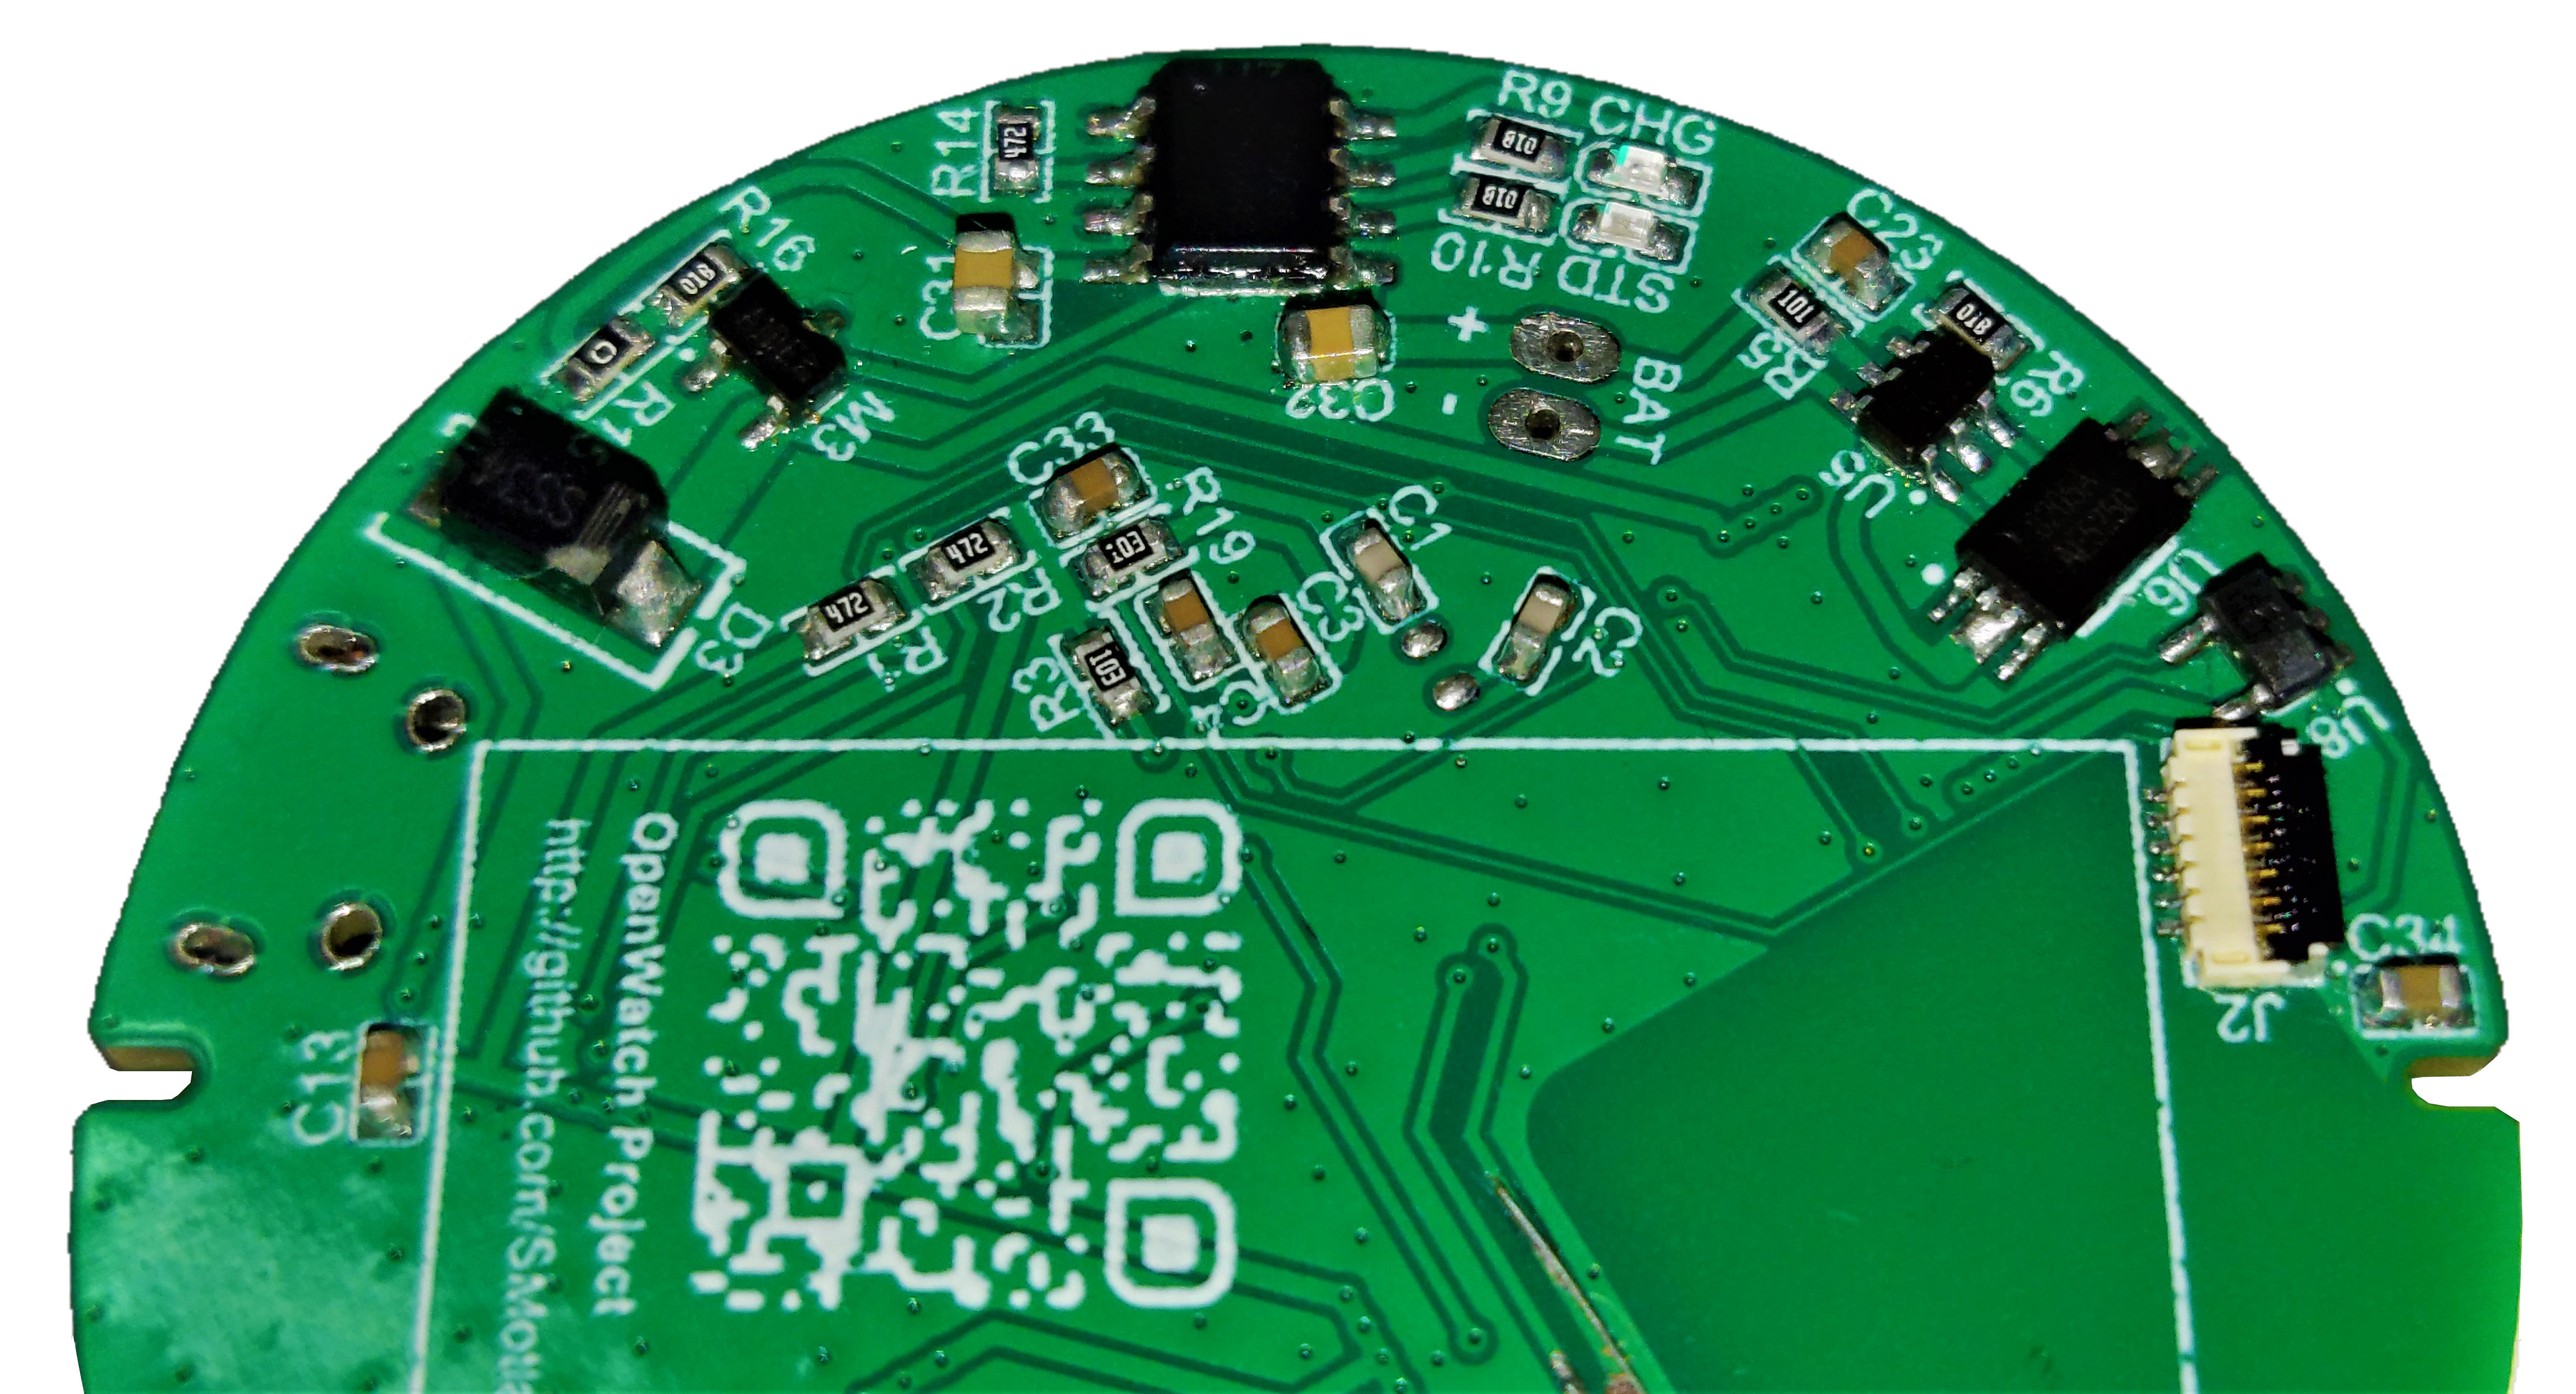
\includegraphics[width=0.5\linewidth]{charge_real}
		\caption{مونتاژ شده روی برد پروژه به همراه جای باتری}
		%\label{fig:vib_real}
	\end{subfigure}
	\caption{تصاویر بخش تغذیه}
	\label{fig:charge}
\end{figure}

دو عدد \lr{LED} به رنگ‌های قرمز و آبی به آیسی شارژ متصلند که در صورت وصل شدن ساعت به شارژر روشن می‌شوند. قرمز برای هنگامی است که باتری در حال شارژ است، آبی برای هنگامی که باتری به طور کامل شارژ شده است.

برای قرائت مقدار شارژ باتری، از یک تقسیم مقاومتی با نسبت سه چهارم (به صورت دقیق 76.0) استفاده شده است که ولتاژ حداکثر 3.4 ولتی باتری را به 3.3 ولت می‌رساند که توسط مبدل آنالوگ به دیجیتال\footnote{\lr{ADC (Analog to Digital Converter)}} قابل خواندن است.

\section{کلیدهای لمسی}
بر روی بدنه‌ی ساعت و زیر صفحه‌ی اصلی، چهار سیم‌پیچ تعبیه شده است که باید بتوان با لمس آن‌ها، با ساعت تعامل کرد و به آن ورودی داد. برای راه‌اندازی این کلیدها از یک آیسی به نام \lr{BS14A-1} استفاده شده است. این آیسی ساخت شرکت \lr{Holtek} است و یکی از بهترین گزینه‌ها برای راه‌اندازی کلید لمسی است. شکل \ref{fig:touch_image} تصویر این موتور و شکل \ref{fig:touch_real} تصویر آن را بر روی \pcbf ساعت نشان می‌دهد.

\begin{figure}[h]
	\centering
	\begin{subfigure}{0.35\textwidth}
		\centering
		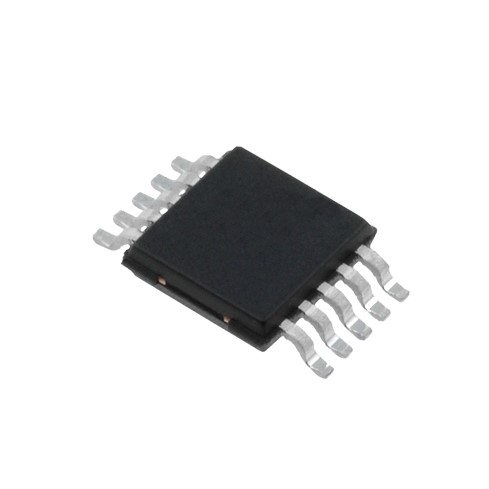
\includegraphics[width=\linewidth]{touch_image}
		\caption{جداگانه}
		\label{fig:touch_image}
	\end{subfigure}
	\begin{subfigure}{0.4\textwidth}
		\centering
		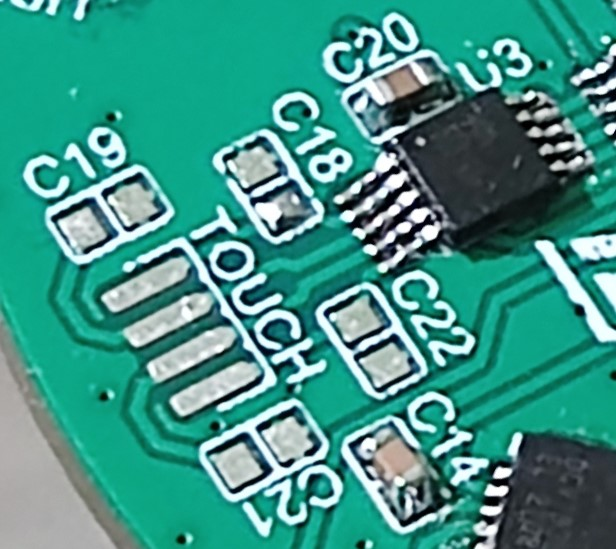
\includegraphics[width=\linewidth]{touch_real}
		\caption{مونتاژ شده روی برد پروژه}
		\label{fig:touch_real}
	\end{subfigure}
	\caption{تصاویر بخش کلیدهای لمسی}
	%	\label{fig:hc05}
\end{figure}

شکل \ref{fig:sch-touch} شماتیک مداری بخش کلیدهای لمسی را نشان می‌دهد. این آیسی ده پایه است. دو پایه برای تغذیه دارد، 4 پایه برای اتصال به کلیدها و 4 پایه برای اتصال به پردازنده. برای تنظیم حساسیت کلیدها می‌توان از خازن‌هایی موازی کلیدها بهره برد. در اینجا خازنی روی برد قرار نگرفته است زیرا نیازی به کاهش حساسیت نبود.

\begin{figure}[h]
	\centering
	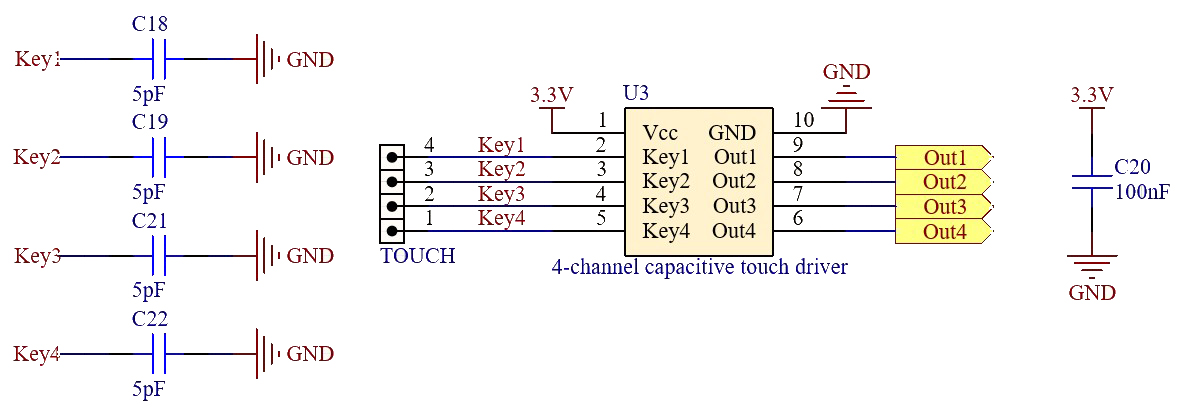
\includegraphics[width=0.9\textwidth]{sch_touch}
	\caption{شماتیک مربوط به بخش کلیدهای لمسی}
	\label{fig:sch-touch}
\end{figure}

\section{بازر}
برای ایجاد صدا و هشدارهای صوتی در ساعت، از یک بازر غیرفعال\footnote{\lr{Passive}} استفاده شده است. بازرهای پسیو، بازرهایی هستند که نوسان‌ساز \footnote{\lr{Oscillator}} داخلی ندارند و تنها با خاصیت پیزوالکتریک \footnote{\lr{Piezoelectric}} کار می‌کنند. بدین صورت که اگر ولتاژ به آن اعمال شود، صفحه‌ی آن جابجا می‌شود و با قطع ولتاژ به مکان اولیه باز می‌گردد.

حال اگر این قطع و وصل ولتاژ با فرکانس مشخصی صورت گیرد، بازر نیز صدایی با همان فرکانس تولید می‌کند. بدیهی است که هارمونیک‌های بالاتر نیز در این صدا وجود دارد زیرا موج ورودی به بازر مربعی است؛ اما فرکانس غالب همان فرکانس اصلی موج مربعی خواهد بود. شکل \ref{fig:buz_image} تصویر بازر و شکل \ref{fig:buz_real} تصویر آن را بر روی \pcbf ساعت نشان می‌دهد.

\begin{figure}[h]
	\centering
	\begin{subfigure}{0.45\textwidth}
		\centering
		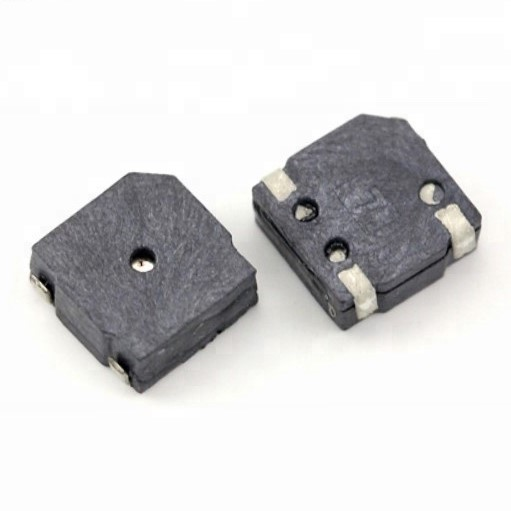
\includegraphics[width=\linewidth]{buz_image}
		\caption{جداگانه}
		\label{fig:buz_image}
	\end{subfigure}
	\begin{subfigure}{0.4\textwidth}
		\centering
		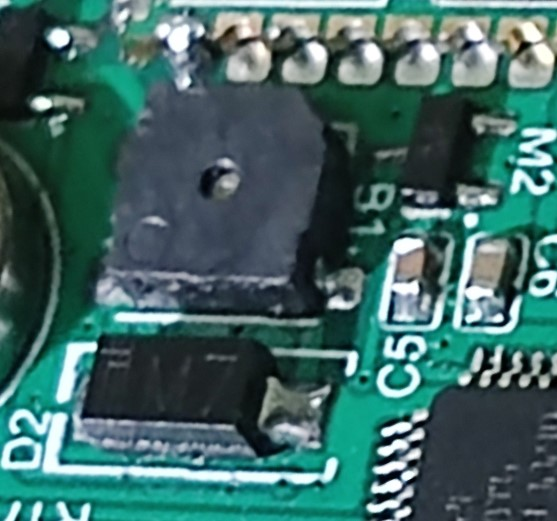
\includegraphics[width=\linewidth]{buz_real}
		\caption{مونتاژ شده روی برد پروژه}
		\label{fig:buz_real}
	\end{subfigure}
	\caption{تصاویر بازر}
	%	\label{fig:hc05}
\end{figure}

شکل \ref{fig:sch-buz} شماتیک مداری بخش بازر را نشان می‌دهد. برای راه‌اندازی بازر و تولید صدا، از یک سوییچ ماسفت برای قطع و وصل ولتاژ استفاده شده است. دیودی که با بازر موازی شده از ورود جریان برگشتی آن به ماسفت هنگام قطع و وصل ولتاژ جلوگیری می‌کند. برای کنترل فرکانس صدا می‌توان از اعمال موج \lr{PWM} به بازر بهره برد. لذا پایه‌ی فرمان این مدار به خروجی \lr{PWM} تایمر 3 در پردازنده متصل شده است.

\begin{figure}[h]
	\centering
	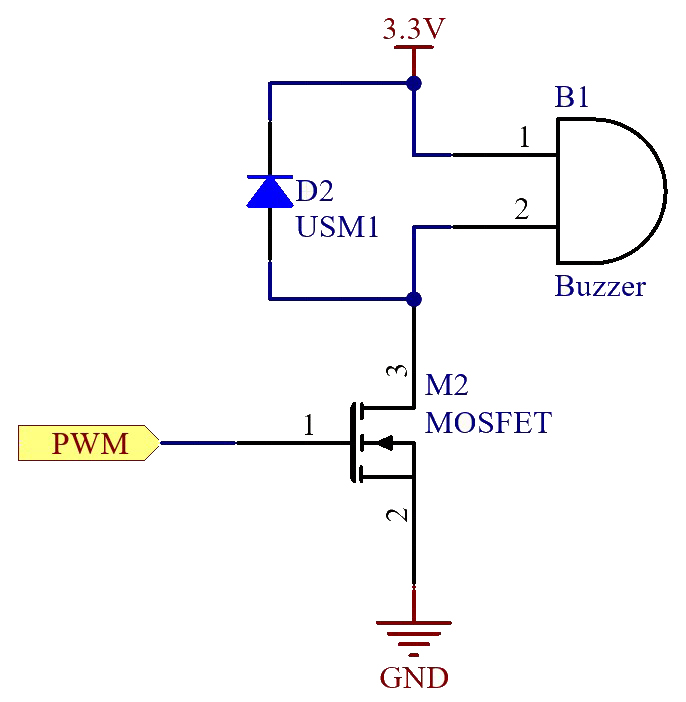
\includegraphics[width=0.45\textwidth]{sch_buz}
	\caption{شماتیک مربوط به بخش بازر}
	\label{fig:sch-buz}
\end{figure}

\section{موتور ایجاد لرزش}
برای ایجاد لرزش\footnote{\lr{Vibration}} در ساعت، مشابه تلفن‌های همراه، از یک موتور مخصوص استفاده شده است. موتورهای ایجاد لرزش معمولا یک موتور \lr{DC} ساده هستند که یک بار نامتقارن به آن‌ها متصل است. از آنجا که مرکز جرم این بار خارج از شفت موتور است، چرخش آن باعث ایجاد گشتاوری دوار می‌شود که لرزش را ایجاد می‌کند. شکل \ref{fig:hc05_image} تصویر این موتور و شکل \ref{fig:hc05_real} تصویر آن را بر روی \pcbf ساعت نشان می‌دهد.

\begin{figure}[h]
	\centering
	\begin{subfigure}{0.4\textwidth}
		\centering
		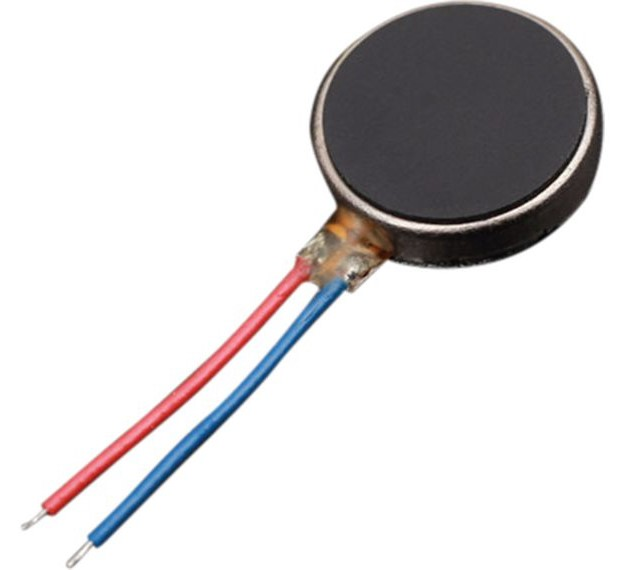
\includegraphics[width=0.75\linewidth]{vib_image}
		\caption{جداگانه}
		\label{fig:vib_image}
	\end{subfigure}
	\begin{subfigure}{0.5\textwidth}
		\centering
		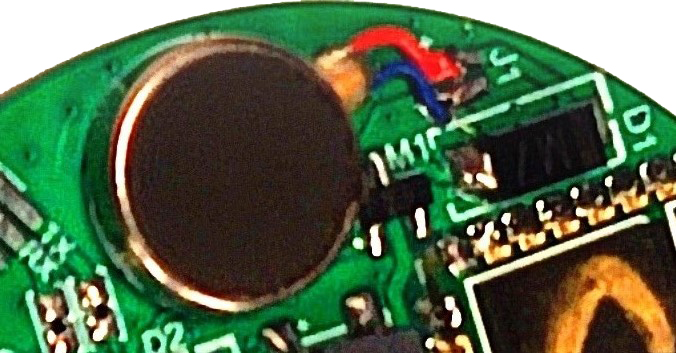
\includegraphics[width=\linewidth]{vib_real}
		\caption{مونتاژ شده روی برد پروژه}
		\label{fig:vib_real}
	\end{subfigure}
	\caption{تصاویر موتور ایجاد لرزش}
	%	\label{fig:hc05}
\end{figure}

شکل \ref{fig:sch-vib} شماتیک مداری بخش ایجاد لرزش را نشان می‌دهد. این موتور برای کار به 90 میلی‌آمپر جریان الکتریکی احتیاج دارد. طبیعتا پردازنده نمی‌تواند این جریان را تأمین کند. لذا از یک کلید ماسفت برای قطع و وصل موتور استفاده شده است. دیودی که با موتور موازی شده از ورود جریان برگشتی موتور به ماسفت هنگام خاموش شدن موتور جلوگیری می‌کند. برای کنترل سرعت موتور می‌توان از اعمال موج \lr{PWM}\footnote{\lr{Pulse Width Modulation}} به موتور بهره برد. لذا پایه‌ی فرمان این مدار به خروجی \lr{PWM} تایمر 1 در پردازنده متصل شده است.

\begin{figure}[h]
	\centering
	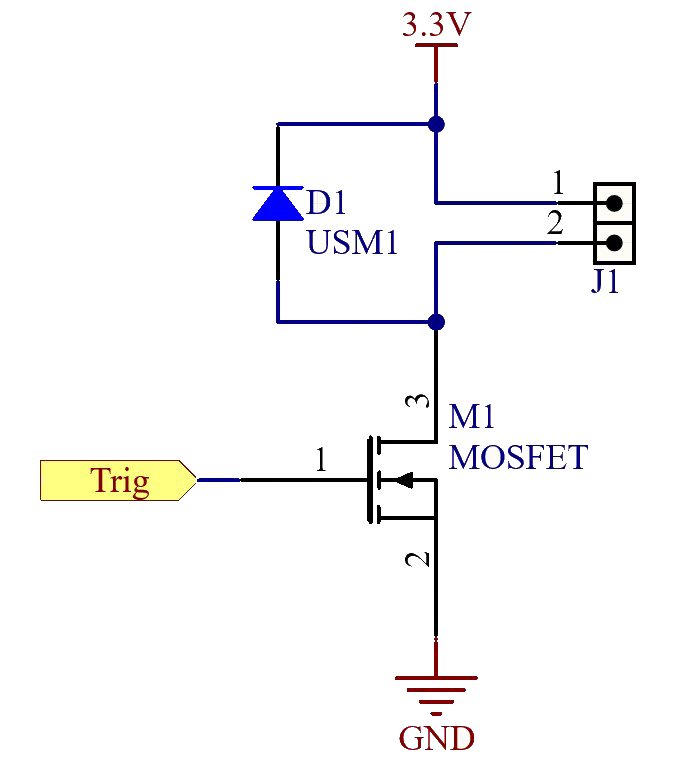
\includegraphics[width=0.45\textwidth]{sch_vib}
	\caption{شماتیک مربوط به بخش ایجاد لرزش}
	\label{fig:sch-vib}
\end{figure}



